\documentclass{VEA}
\usepackage{amsmath}
\usepackage{graphicx}
\usepackage{tabularray}
\usepackage{float}
\usepackage{url}
\usepackage{makecell}
\graphicspath{ {./images/} }

%% Pakotne lai saliktu automātisku figūru skaitīšanu
\usepackage{totcount}

%% Precīzu attālumu izveide starp tekstiem vienā rindā
\usepackage{tabto}

%% Lapu numuriem labajā pusē
\usepackage{fancyhdr}
\fancypagestyle{plain}{%
\fancyhf{} % clear all header and footer fields
\fancyfoot[RO,RE]{\thepage} %RO=right odd, RE=right even
\renewcommand{\headrulewidth}{0pt}
\renewcommand{\footrulewidth}{0pt}}

\newcounter{nofappendices}
\setcounter{nofappendices}{0}
\regtotcounter{nofappendices}

\newtotcounter{fignum}
\def\oldfigure{} \let\oldfigure=\figure
\def\figure{\stepcounter{fignum}\oldfigure}

%defineejam atsauču skaitītāju
\newtotcounter{citnum}
\def\oldbibitem{} \let\oldbibitem=\bibitem
\def\bibitem{\stepcounter{citnum}\oldbibitem}

\begin{document}
\pagenumbering{gobble}
%%%% Titullapas sākums
%% Sarakstam visus mainīgos
%% Mainīgie titullapai, defAutors tiek izmantots arī galvojumā
\def\defAutors{Matīss Kalniņš}
\def\defAugstskola{Ventspils Augstskola}
\def\defFakultate{Informācijas tehnoloģiju fakultāte}
\def\defSProgrammas{bakalaura studiju programmas \\
„Datorzinātnes” 
}
\def\defStudents{3.  kursa students \\
	      \defAutors}
\def\defMatrikulasNr{23020018}
\def\defDarbaNosaukums{Ziņu portālu rakstu klasifikācija (ar mašīnmācīšanās algoritmiem)}
\def\defDarbaNosaukumsEN{Classification of news articles (with machine learning algorithms)}
\def\defDarbaVeids{Bakalaura darbs}
\def\defFakultatesDekans{doc. Dr.sc.comp. Vairis Caune}
\def\defZinVaditajs{Mg.sc.comp. Agris Blūms}
\def\defGads{2024}
 %šeit pārdefinējam savus mainīgos
%%%% Titullapas sākums
\begin{titlepage}
\begin{center}
\textbf{\MakeUppercase{
\defAugstskola\\
\defFakultate}}\\
\vspace{2em}
\textbf{\MakeUppercase{\defDarbaVeids}}\\
\vspace{2em}
{\LARGE \textbf{\defDarbaNosaukums}}\\
\vspace{2em}
\begin{tabular}{@{}r@{}l@{}}
\parbox[c]{0.4\textwidth}{Autors:}&
\parbox[t]{0.6\textwidth}{
\defAugstskola s\\
\defFakultate s\\
\defSProgrammas\\
\defStudents \\
Matrikulas~Nr. \defMatrikulasNr\vspace{0.7em}\\
\mbox{}\hrulefill\vspace{-0.4em}\\
{\scriptsize(paraksts)}\vspace{2em}} \\
\parbox[c]{0.4\textwidth}{Fakultātes dekāns:}&
\parbox[t]{0.6\textwidth}{
\defFakultatesDekans\vspace{.7em}\\
\mbox{}\hrulefill\vspace{-0.4em}\\
{\scriptsize(paraksts)}\vspace{2em}} \\
\parbox[c]{0.4\textwidth}{Zinātniskais vadītājs:}&
\parbox[t]{0.6\textwidth}{
\defZinVaditajs\vspace{.7em}\\
\mbox{}\hrulefill\vspace{-0.4em}\\
{\scriptsize(paraksts)}\vspace{2em}} \\
\parbox[c]{0.4\textwidth}{Recenzents:} & \vspace{.7em}\\
\multicolumn{2}{@{}c@{}}{
\mbox{}\hrulefill
}\vspace{-0.4em}\\
\multicolumn{2}{@{}l@{}}{
{\scriptsize(Ieņemamais amats, zinātn. nosaukums,
vārds, uzvārds)}
}\vspace{.7em}\\
&\mbox{}\hrulefill\vspace{-0.4em}\\
&{\scriptsize(paraksts)}\\
\end{tabular}
\vfill
Ventspils, \defGads
\end{center}
\end{titlepage}
 %pievienota titullapa, kura izveidota atsevišķā failā

\tableofcontents
\clearpage


%%%% Nodaļa bez numerācijas
\pagestyle{plain}
\pagenumbering{arabic} % sākam numurēt lapas
\setcounter{page}{4}
\chapter*{Anotācija}
%%%% Lai uzrādītos satura rādītājā
\addcontentsline{toc}{chapter}{Anotācija}

\begin{tabular}{@{}r@{}l@{}}
\parbox[c]{0.3\textwidth}{\textbf{Darba nosaukums:}}&
\parbox[t]{0.65\textwidth}{\defDarbaNosaukums} \\
\parbox[c]{0.3\textwidth}{\textbf{Darba autors:}}&
\parbox[t]{0.65\textwidth}{\defAutors} \\
\parbox[c]{0.3\textwidth}{\textbf{Darba vadītājs:}}&
\parbox[t]{0.65\textwidth}{\defZinVaditajs} \\
\parbox[c]{0.3\textwidth}{\textbf{Darba apjoms:}}&
\parbox[t]{0.65\textwidth}{\textcolor{black}{\pageref{LastPage}} lpp, 6~tabulas,  \total{fignum}~attēli, 12~formulas, \total{citnum}~bibliogrāfiskās norādes, \total{nofappendices}~pielikumi} \\
\parbox[c]{0.3\textwidth}{\textbf{Atslēgas vārdi:}}&
\parbox[t]{0.65\textwidth}{Dabiskās valodas apstrāde, mašīnmācīšanās, tekstu klasifikācija} \\
&\\
\end{tabular}

Bakalaura darbā ir aprakstīta dabīgās valodas apstrāde un kā mašīnmācīšanās metodes var palīdzēt risināt teksta klasifikācijas problēmu, konkrēti apskatot tieši ziņu klasifikāciju latviešu valodas rakstiem.

Darba ietvaros tiek ievākta rakstu kopa no ziņu portāliem un pārbaudīts kāda pieeja sniedz augstāko precizitāti teksta klasifikācijai latviešu valodā. Tiek izvērtētas un salīdzinātās dažādas pazīmju ģenerēšanas pieejas un apmācības algoritmi (naivā Bajesa metode, loģistiskā regresija, lēmumu koki, atbalsta vektora mašīnas, neironu tīkli).

Papildus apskatītas dažādas atvērtā pirmkoda bibliotēkas mašīnmācīšanās problēmu risināšanai kā scikit-learn un Tensorflow, to praktiskais pielietojums dabīgo valodu apstrādei.


\clearpage

\selectlanguage{english}
\chapter*{Abstract}
%%%% Lai uzrādītos satura rādītājā
\addcontentsline{toc}{chapter}{Abstract}

\begin{tabular}{@{}r@{}l@{}}
\parbox[c]{0.3\textwidth}{\textbf{The title:}}&
\parbox[t]{0.65\textwidth}{\defDarbaNosaukumsEN} \\
\parbox[c]{0.3\textwidth}{\textbf{Author:}}&
\parbox[t]{0.65\textwidth}{\defAutors} \\
\parbox[c]{0.3\textwidth}{\textbf{Academic Advisor:}}&
\parbox[t]{0.65\textwidth}{\defZinVaditajs} \\
\parbox[c]{0.3\textwidth}{\textbf{The volume of the work:}}&
\parbox[t]{0.65\textwidth}{\textcolor{black}{\pageref{LastPage}} pages, 6~tables,  \total{fignum}~images, 12~equations, \total{citnum}~literature sources, \total{nofappendices}~appendices} \\
\parbox[c]{0.3\textwidth}{\textbf{Keywords:}}&
\parbox[t]{0.65\textwidth}{ Natural language processing, machine learning, text classification} \\
&\\
\end{tabular}

The bachelor thesis describes natural language processing and how machine learning methods can help to resolve text classification problems, focusing specifically the classification of news articles in the Latvian language.

As part of this work a data set of articles is gathered from Latvian news websites and the best approach is researched for achieving the highest accuracy of Latvian text classification. Various feature generation approaches and learning algorithms (e.g. Naïve Bayes, logistic regression, decision trees, support vector machines, neural networks) are evaluated and compared.

In addition, various open source libraries for machine learning as scikit-learn and Tensorflow along with their practical applications for natural language processing are explored as part of this work.

\selectlanguage{latvian}

%------------------------------------------------APZĪMĒJUMI---------------------------------------------------------
%%%% Nodaļa bez numerācijas
\chapter*{Izmantotie saīsinājumi un termini}
\addcontentsline{toc}{chapter}{Izmantotie saīsinājumi un termini}

\textbf{DVA} - Dabisko valodu apstrāde (angliski - natural language processing)

\textbf{TF-IDF} - Terminu biežums - inversais dokumentu biežums (angliski - term frequency - inverse document frequency)

\textbf{Epoha}  - Apmācības periods. Apmācības procesa daļa, kurā neironu tīkls tieši vienu reizi tiek apmācīts uz visiem apmācības piemēriem (no angliskā termina - epoch).

\textbf{PA} - pareiza atbilsme (angliski - true positive)

\textbf{PA} - pareiza atbilsme (angliski - true positive)

\textbf{PN} - pareiza neatbilsme (angliski - true negative)

\textbf{KA} - kļūdaina atbilsme (angliski - false positive)

\textbf{KN} - kļūdaina neatbilsme (angliski - false negative)

\chapter*{Ievads} % * nepieliks numuru pie nosaukuma
\addcontentsline{toc}{chapter}{Ievads}
Mūsdienās internets ir kļuvis par galveno informācijas avotu lielai daļai cilvēku, kuri ikdienā ar dažādu mediju palīdzību caur to gūst informāciju par jaunākajām aktualitātēm savā rajonā, valstī un pasaulē. Svarīga loma informācijas iegūšanā un izplatīšanā ir arī pareizai teksta klasifikācijai, lai šī informācija sasniegtu vēlamo lasītāju. Pārsvarā problēma tiek atrisināta autoram klasificējot savu darbu jau izveides procesā, tomēr bieži ar to vien nepietiek – tiek pārpublicēti raksti no ārējiem resursiem, mainās kategoriju iedalījums, aktuālas kļūst jaunas tēmas u.t.t. Lai gan arī šādos gadījumos klasifikāciju iespējams darīt manuāli, pie liela informācija apjoma kļūst jēgpilni šo klasifikāciju automatizēt ar mašīnmācīšanās algoritmiem, ietaupot laiku un resursus. 

Pirms darba uzsākšanas, veicot izpēti par labākajiem algoritmiem tekstu klasifikācijai, konstatēts, ka viennozīmīgi labākā pieeja problēmas risināšanai neekstistē, optimālā pieeja atkarīga no daudziem faktoriem – gan no dažādām datu kopas īpašībām (valoda, temati, tekstu garumi, valodas stili u.t.t.), gan klašu skaita klasifikācijā, gan pielietotajām priekšapstrādes metodēm, gan cik labi algoritmi mērogojas ar dažādiem datu kopu izmēriem. Līdzīgu ieskatu vispārējā problēmvidē sniedz arī “Papers With Code”\footnote{https://paperswithcode.com/task/text-classification}, kas apkopo ar mašīnmācīšanos saistītās publikācijas un tajos iekļauto modeļu veiktspējas rādītājus, to starpā arī 1091 publikācijas par tekstu klasifikāciju. Šajā resursā iespējams novērot, ka pēdējos gados labākos rezultātus pārsvarā, bet ne vienmēr, sniedz lielo valodu modeļi kā XLNet un BERT. Konkrēti šos iepriekš apmācītos modeļus nav iespējams pielietot latviešu tekstu klasifikācijai - šie modeļi ir apmācīti uz ļoti liela angļu valodas tekstu apjoma - BERT gadījumā 3,3 miljardu vārdu korpusa, XLNet gadījumā - jau krietni lielāka. Salīdzinoši lielākais latviešu valodas korpuss šobrīd (LVK2022\footnote{https://korpuss.lv/id/LVK2022}) satur tikai 101 miljonu vārdu. Nākošo labāko algoritmu veiktspējas atšķirības kļūst mazāk izteiktas – labus rezultātus sasniedz gan dažādas rekurento neironu tīklu arhitektūras (LSTM balstīti modeļi), gan konvolūcijas neironu tīkli, gan arī vienkāršākas pieejas kā atbalsta vektora mašīnas. Šo secinājumu rezultātā izlemts izpētīt cik labi klasifikāciju iespējams veikt ar plašu spektru ar klasifikācijas metodēm – sākot no vienkāršiem klasifikācijas algoritmiem kā Naivā Bajesa metode, atbalsta vektora mašīnas u.c., turpinot ar dažādām neironu tīklu arhitektūrām, kā arī pielāgojot BERT arhitektūrā balstīto LVBERT modeli. 

Darba mērķis ir izveidot mašīnmācīšanās modeli, kas ar augstu precizitāti spētu klasificēt ziņu portālu rakstus latvieu valodā. Lai sasniegtu šo mērķi, tiek izvirzīti sekojoši uzdevumi:
\begin{enumerate}
\item Veikt literatūras izpēti par mašīnmācīšanos un tekstu klasifikāciju
\item Izveidot rāpuli ar kura palīdzību izgūt un marķēt ziņu portālu rakstus, pielietojamus modeļu apmācībā
\item Implementēt dažādus mašīnmācīšanās algoritmus tekstu klasifikācijai
\item Izpētīt kā dažādas pazīmju ģenerēšanas pieejas ietekmē klasifikācijas rezultātus
\item Veikt precizitātes novērtējumus un salīdzināt cik labi dažādos algoritmos balstīti modeļi spēj veikt latviešu valodas tekstu klasifikāciju
\end{enumerate}

Lai veiktu algoritmu implementēšanu un analīzi tiks izmantota programmēšanas valoda Python un plaši pielietotas bibliotēkas mašīnmācīšanās problēmu risināšanai (scikit-learn, Tensorflow).

Darbs sastāv no 4 nodaļām. Pirmajā nodaļā tiek apskatīta dabiskās valodas apstrāde un mašīnmācīšanās, pamatjēdzieni uz kuriem balstās nākošo nodaļu saturs.

Otrajā nodaļā uzsvars tiek likts uz pazīmju ģenerēšanas aprakstu un literatūras izpēti par to. Šis ir svarīgs solis pirms mašīnmācīšanās algoritmu pielietošanas, pārvēršot teksta informāciju apstrādei piemērotā formā un ietekmējot to cik veiksmīgu modeli būs iespējams izveidot.

Trešajā nodaļā konkrēti tiek apskatīti dažādi izplatītākie algoritmi ar kuriem veikt teksta klasifikāciju – sākot no vienkāršākām pieejām kā atbalsta vektora mašīnas, turpinot ar neironu tīkliem un lielajiem valodas modeļiem kā BERT.

Ceturtajā nodaļā tiek apskatīta rāpuļa un klasifikācijas modeļu praktiskā izveide, cik labi dažādi modeļi spēja sasniegt vēlamo rezultātu.


%------------------------------------------------DARBS--------------------------------------------------------------

\chapter{Mašīmācīšanās valodas apstrādē}
\section{Dabiskās valodas apstrāde}
Dabiskā valodas apstrāde jeb NLP apvieno datorlingvistiku - uz likumiem balstītu cilvēka valodas modelēšanu - ar statistikas un mašīnmācīšanās modeļiem, lai datori un digitālās ierīces varētu atpazīt, saprast un ģenerēt tekstu un runu \cite{ibmMachineLearning}.

Cilvēku valodai ir sarežģīta uzbūve, kuru dažkārt ir grūti aprakstīt. Par piemēru ņemot problēmu par nodoma izprašanu - valodas stili kā sarkasms, homonīmi, idiomas, metaforas, dažādas sintaktiskās konstrukcijas, tie visi apgrūtina šādu uzdevumu. Lai palīdzētu datoram izprast cilvēku valodu, tiek veikti dažādi dabiskās valodas apstrādes pamatuzdevumi, ieskaitot arī tālāk norādītos.
\begin{itemize}
\item Balss atpazīšana: balss datu pārveide teksta datos. Cilvēku runas veids (dažādas valodas, akcenti, runas temps, intonācijas, nepareiza gramatika, neskaidra izruna) un tā daudzveidība padara šo par īpaši sarežģītu problēmu
\item Nosaukto entītiju atpazīšana: nosaukumu atpazīšana un iedalīšana kategorijās, piemēram, personvārdos, datumos, atrašanās vietās
\item Semantiskā analīze: vārdiem ar daudzām nozīmēm nepieciešams analizēt kontekstu, lai spētu noteikt vārda nozīmi konkrētajā lietojumā
\item Lemmatizācija: vārdu pārveidošana pamatformā
\item Tokenizācija: teksta sadalīšanas process vārdos vai frāzēs
\item Morfoloģiskā marķēšana: marķējumu piešķiršana vārda daļām (saknes, priedēkļi galotnes u.c. daļas)
\item Runas daļu marķēšana: marķējumu piešķiršana vārdiem, atkarībā no to vārdšķiras (lietvārds, darbības vārds, saiklis u.c.)
\item Sintakses parsēšana: teikumu gramatiskās struktūras analīze
\end{itemize}

Pielietojot daļu no šīm komponentēm iespējami sarežģītāki pielietojumi teksta apstrādei – klasifikācijai, tekstu kopsavilkumu veidošanai, noskaņojuma analīzei, mašīntulkošanai, čatbotu izveidei. 

Sākotnējās DVA sistēmas balstījās uz manuāli izstrādātiem noteikumiem, taču šīs sistēmas ir ierobežotas ar savu nespēju apstrādāt cilvēku valodu daudzveidību un sarežģītību, kā rezultātā DVA sistēmas mūsdienās bieži tiek veidotas tieši ar mašīnmācīšanās iesaisti.

\section{Mašīnmācīšanās}
Mašīnmācīšanās ir mākslīgā intelekta nozare, kas nodarbojas ar datorprogrammu izstrādi, kuras, izmantojot algoritmus un statistikas modeļus, mācās no datiem un uzlabo savu precizitāti. Toms Mičels savukārt apraksta mašīnmācīšanās jomu, izvirzot centrālo jautājumu, ko tā pēta: "Kā mēs varam izveidot datoru sistēmas, kas automātiski uzlabojas, iegūstot pieredzi, un kādi ir pamatlikumi, kas nosaka visus mācīšanās procesus?" \cite{definitionML}.

Induktīvā mācīšanās ir mašīnmācīšanās apakšnozare, kas specifiski nodarbojas ar modeļu mācīšanos no novērojumiem. Šajā nozarē mācīšanās uzdevumi bieži tiek raksturoti, pamatojoties uz atgriezenisko saiti, kas tiek sniegta apmācības veicējam \cite{russel2010} tālāk norādītos veidos.

\begin{itemize}
\item Uzraudzīta mācīšanās: apmācības procesā tiek sniegts vēlams izvads katram novērojumam. Mērķis ir iemācīties funkciju, kas paredz pareizo izvades vērtību brīdī kad tiek sniegts iepriekš neredzēts novērojums.
\item Neuzraudzīta mācīšanās: apmācības laikā netiek sniegts izvads. Mērķis ir atklāt paraugus un regulāras pazīmes datos.
\item Stimulētā mācīšanās: Īpašs uzraudzītās mācīšanās gadījums, kur apmācības laikā tiek sniegta atlīdzība pēc katras darbības.
\end{itemize}

Uzraudzītas mācīšanās gadījumus, kad uzdevums ir iemācīties diskrēti vērtētu funkciju, sauc par klasifikāciju. Uzdevums, kad jāiemācās nepārtraukti vērtēta funkcija, tiek saukts par regresiju. Savukārt klasterošana ir neuzraudzītās mācīšanās uzdevums, kas atrod līdzīgu objektu grupas datu kopā. Šī darba ietvaros tiek apskatīta tieši klasifikācija.

\pagebreak
\section{Tekstu klasifikācija}

Tekstu klasifikācijas mērķis ir tekstu piesaiste konkrētai klasei, balstoties uz teksta saturu. Šāda klasifikācija ir pielietojama ziņu portālos un citur, kur nepieciešams kategorizēt lielu datu daudzumu. Mašīnmācīšanās algoritmi ļauj rast risinājumu dažādām problēmām, piemēram, ar augstu precizitāti noteikt vai ienākošais e-pasts ir vai nav mēstule. Iespējams arī veikt sentimentu analīzi un noteikt cilvēku attieksmi par kādu konkrētu tematu, piemēram, M. Kandias ir apskatījis kā ar tekstu klasifikācijas palīdzību noteikt negatīvu attieksmi pret likumsargiem, balstoties uz konkrēta lietotāja ierakstiem vietnē YouTube \cite{threatdetectionyoutube}.

\begin{figure}[H]
	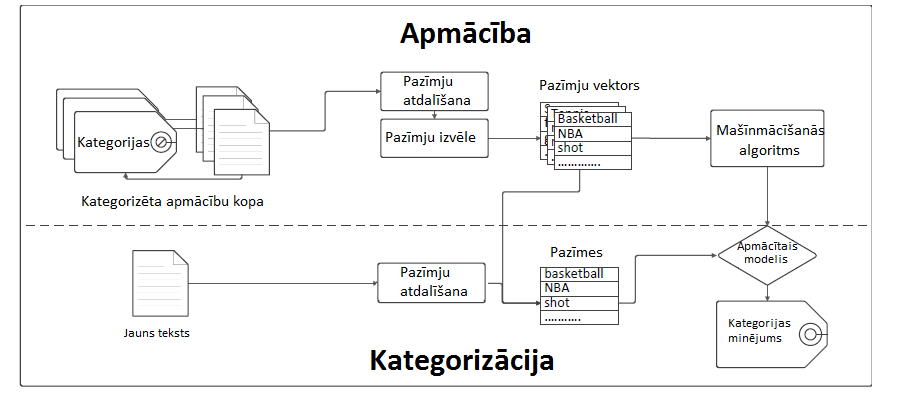
\includegraphics[width=\textwidth]{masinmacisanas}
	\caption{Mašīnmācīšanās tekstu klasifikācijai}
	\label{fig:masinmacisanas}
\end{figure}

Teksta klasifikācijas piemēru ar mašīnmācīšanās pielietojumu iespējams redzēt attēlā  \ref{fig:masinmacisanas}. Pieņemsim, ka dota datu kopa ar sporta ziņām, un risināmā problēma ir - kā klasificēt jaunu dokumentu, piešķirot tam atbilstošā sporta veida marķējumu. Sākumā būs nepieciešami apmācības dokumenti (ar klases marķējumiem) no kuriem mācīties. Tālāk katru ziņu mēs pārveidojam par pazīmju kopu, kuru vektorizētā veidā mēs varam padot tālāk mašīnmācīšanās algoritmam. Ar šo informāciju algoritms izveido modeli, kas var paredzēt iepriekš neredzētu tekstu klases.

\chapter{Pazīmju ģenerēšana}
\section{Tekstu priekšapstrāde}
Pirms iespējams izveidot klasifikācijas modeli, nepieciešams veikt teksta priekšapstrādi, lai dati būtu pielietojami tālākajā apstrādē. Tas sevī ietver gan dažādu teksta fragmentu atmešanu, gan pārveidošanu formā kuru spētu saprast apmācības algoritmi. Tālāk apskatīti konkrēti priekšapstrādes soļi.

\subsubsection{Vārdu atdalīšana jeb tokenizācija}
Lai tekstu izmantotu klasificēšanā, ir jāspēj atdalīt atsevišķas šī teksta daļas. To iespējams paveikt dažādos veidos – tekstu iespējams sadalīt pa individuāliem vārdiem vai arī  secīgu vārdu grupām. Vārdu atdalīšanai var izmantot dažādus atdalošos simbolus, piemēram atstarpi un jaunas līnijas sākuma simbolu (\textbackslash n’). Tomēr ne visi atdalošie simboli ir viennozīmīgi, piemēram punkts var būt gan kā teikuma beigas, gan kā daļa no konkrētas vērtības (skaitlis 10.5).
Vārdu atdalīšana secīgās vārdu grupās izmanto n-grammas, kas ir n secīgu vārdu un/vai simbolu kopa tekstā. Izmantojot n-grammas, iespējams iegūt plašāku teksta kontekstu no atdalītajiem vārdiem.

\subsubsection{Sakņu atdalīšana un lemmatizācija}
Apstrādājot tekstus, svarīgi ir arī ņemt vērā faktu, ka dažādos tekstos viens un tas pats vārds bieži tiek lietots dažādos locījumos un visbiežāk locījumam nav ietekme uz to vai teksts pieder konkrētai klasei. Svarīgi arī ņemt vērā, ka liels individuālu vārdu atkārtojums dažādos locījumos palielina klasifikācijai nepieciešamo laiku un resursus. Sakņu atdalīšana un lemmatizācija risina šo problēmu, pārvēršot vārdus dažādos locījumos vienādā formā. Sakņu atdalīšanas gadījumā tiek mēģināts nodzēst vārdu galotnes / piedēkļus (saulei - saul, saulīte - saul), balstoties uz valodas likumsakarībām vārda daļu atpazīšanai. Lemmatizācijas gadījumā vārdi tiek pārveidoti to pamatformā (saulei - saule, saulīte - saule), šādai apstrādes metodei nepieciešama krietni sarežģītāka morfoloģijas izpratne.

\subsubsection{Stopvārdu dzēšana}
Bieži vien noderīga ir arī tā sauktā stopvārdu (angliski - stopwords) dzēšana no apstrādāmajiem datiem. Tie ir vārdi kuri neietekmē teksta saturu un to biežais lietojums var atstāt negatīvu ietekmi uz klasifikācijas akurātumu. Latviešu valodā piemērs šādiem vārdiem būtu palīgvārdi, kuri ietver saikļus (un, bet, vai u.c.), prievārdus (uz, no u.c.), partikulas (arī, diezin, gan u.c.).

\section{Vektorizācija}
Teksta vektorizācija ir process, kurā teksta informācija tiek pārveidota skaitļu formā, ko tālāk var izmantot mašīnmācīšanai. Šis solis ir būtisks, jo mašīnmācīšanās algoritmi strādā ar skaitļiem, bet teksta dati ir paši par sevi neskaitliski. Teksta vektorizācijai ir vairākas metodes, populārākās no tām apskatītas zemāk.

\subsubsection{Vārdu maiss}
Vārdu maiss – tā ir nesakārtota vārdu kopa, kur vārdu secība tiek ignorēta, saglabājot tikai vārdu biežumu dokumentā \cite{speechandlanguageproc}. Teksts tiek pārveidots vektorā, kur katram unikālam vārdam dokumentā tiek piešķirts indekss, kā vērtību indeksā norādot konkrētā vārda biežumu. 

Lai ilustrētu šādu pieeju, pielietojam to uz diviem teikumiem:

1. Kaķis devās medīt peles

2. Kaķis ātri skrēja, peles ātri bēga

Rezultātā iegūstot vektorus teikumiem kā \ref{tab:vardu_maiss} tabulā.
\begin{table}[H]
\centering
\caption{\label{tab:vardu_maiss}}
\textbf{Vārdu maisa vektori diviem teikumiem\\}
\begin{tabular}{|l|l|l|l|l|l|l|l|}
\hline
           & kaķis & devās & medīt & peles & ātri & skrēja & bēga \\ \hline
1. teikums & 1     & 1     & 1     & 1     & 0    & 0      & 0    \\ \hline
2. teikums & 1     & 0     & 0     & 1     & 2    & 1      & 1    \\ \hline
\end{tabular}
\end{table}

Ar šo pieeju mēs veicam šādus pieņēmumus:
\begin{itemize}
\item Tekstu iespējams analizēt, ignorējot vārdu / tekstvienību secību.
\item Nepieciešams zināt tikai kuri vārdi / tekstvienības atrodas tekstā un cik bieži tie atkārtojas.
\end{itemize}

Plašāka konteksta izgūšanai no teksta, iespējams veidot vektorus, kur katram indeksam atbilst vairāku secīgu vārdu kombinācija jeb n-gramma. Piemēram, izvēloties n-grammas ar garumu 2 (bigrammas), iepriekš apskatīto teikumu vektori izskatītos kā \ref{tab:vardu_maiss_bigramma} tabulā.

\begin{table}[H]
\centering
\caption{\label{tab:vardu_maiss_bigramma}}
\textbf{Bigrammu maisa vektori diviem teikumiem\\}
\begin{tabular}{|l|l|l|l|l|l|l|l|l|}
\hline
 & \begin{tabular}[c]{@{}l@{}}kaķis\\ devās\end{tabular} & \begin{tabular}[c]{@{}l@{}}devās\\ medīt\end{tabular} & \begin{tabular}[c]{@{}l@{}}medīt\\ peles\end{tabular} & \begin{tabular}[c]{@{}l@{}}kaķis\\ ātri\end{tabular} & \begin{tabular}[c]{@{}l@{}}ātri\\ skrēja\end{tabular} & \begin{tabular}[c]{@{}l@{}}skrēja\\ peles\end{tabular} & \begin{tabular}[c]{@{}l@{}}peles\\ ātri\end{tabular} & \begin{tabular}[c]{@{}l@{}}ātri\\ bēga\end{tabular} \\ \hline
1. teikums & 1 & 1 & 1 & 0 & 0 & 0 & 0 & 0 \\ \hline
2. teikums & 0 & 0 & 0 & 1 & 1 & 1 & 1 & 1 \\ \hline
\end{tabular}
\end{table}

\subsubsection{TF-IDF}
Terminu biežums - inversais dokumentu biežums (angliski, saīsināti - TF-IDF) ir vektorizācijas paveids ko izmanto, lai novērtētu termina (vārda) svarīgumu tekstā attiecībā uz dokumentu kopu (korpusu) \cite{manning_raghavan_schutze_2008}. 

Termina biežums (TF):

Termina biežums nosaka, cik bieži konkrēts termins parādās konkrētā dokumentā. To aprēķina kā attiecību starp termina parādīšanos dokumentā un kopējo terminu skaitu šajā dokumentā. Termina biežuma (TF) formula ir šāda:

\begin{equation}
TF(t, d) = \frac{f(t, d)}{|d|}
\end{equation}

\noindent Kur:
\begin{itemize}
\item \(TF(t, d)\) ir termina biežums terminam \(t\) dokumentā \(d\).
\item \(f(t, d)\) ir termina \(t\) biežums dokumentā \(d\).
\item \(|d|\) ir kopējais terminu skaits dokumentā \(d\).
\end{itemize}

Inversais dokumenta biežums (IDF):
Inversais dokumenta biežums nosaka cik unikāls vai svarīgs ir termins visā dokumentu kopā (korpusā). To aprēķina kā logaritmisku attiecību starp visu dokumentu kopā esošo dokumentu skaitu un dokumentu skaitu, kuros šis termins parādās. Inversās dokumentu biežuma (IDF) formula ir šāda:

\begin{equation}
IDF(t, D) = \log\left(\frac{|D|}{|{d \in D : t \in d}|}\right)
\end{equation}

\noindent Kur:
\begin{itemize}
\item \(IDF(t, D)\) ir termina \(t\) inversais dokumenta biežums kopā \(D\).
\item \(|D|\) ir kopējais dokumentu skaits korpusā.
\item \(|{d \in D : t \in d}|\) ir dokumentu skaits, kas satur terminu \(t\).
\end{itemize}

TF-IDF beigu rezultāts ir termina biežuma (TF) un inversā dokumenta biežuma (IDF) reizinājums:

\begin{equation}
TF\text{-}IDF(t, d, D) = TF(t, d) \times IDF(t, D)
\end{equation}

TF-IDF rezultāts atspoguļo, cik svarīgs ir vārds konkrētajā dokumentā, ņemot vērā visu tekstu kopu. Augstāki TF-IDF vērtējumi tiek piešķirti terminiem, kas bieži parādās dokumentā, bet reti visā kopā. Tas palīdz uzsvērt terminu svarīgumu, kuri ir raksturīgi tieši konkrētiem dokumentiem, vienlaikus samazinot kopīgu terminu nozīmi, kas parādās daudzos dokumentos.

\subsubsection{Vārdlietojuma kartējums}
Vārdlietojuma kartējums (angliski - word embedding) ir jaunāka metode, kur vārdi tiek attēloti kā skaitliski vektori daudzdimensiju telpā. Šie vektori spēj saglabāt informāciju par vārdu kontekstu / nozīmi / saikni ar citiem vārdiem, respektīvi -  vārdi ar līdzīgu nozīmi vai pielietojumu ir attēloti ar vektoriem, kas ģeometriski atrodas tuvu viens otram vektoru telpā. Piemēram, labi apmācītā vārdlietojuma kartējuma modelī vārdi "karalis" un "karaliene" tiek attēloti kā vektori, kas ir tuvu viens otram, norādot to semantisko līdzību \cite{BaeldungEmbedding}. Šāda pieeja tiek vizualizēta \ref{fig:wordembedding} attēlā.

\begin{figure}[H]
	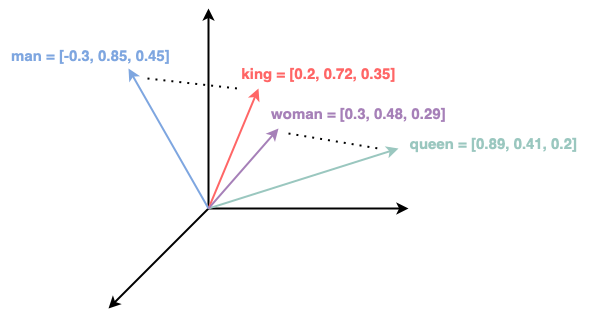
\includegraphics[width=\textwidth]{word_embedding}
	\caption{Vārdlietojuma kartējums vektora telpā \cite{BaeldungEmbedding} }
	\label{fig:wordembedding}
\end{figure}

Vārdlietojuma kartējums ļauj arī veikt dažādas operācijas ar vārdiem vektoru telpā, to skaitā arī  saskaitīšanu un atņemšanu. Piemēram, "karalis - vīrietis + sieviete" varētu izveidot vektoru, kas vektora telpā ir tuvu vārdam "karaliene".

\subsubsection{Pazīmju izvēle}
Iepriekš tika apskatīts kā atlasīt pazīmes no dokumentu kopas. Atkarībā no apskatīto tekstu daudzuma un sarežģītības, rezultātā var tikt iegūts liels pazīmju skaits, kas var apgrūtināt mašīnmācīšanās algoritmu pielietošanu. Pārāk plaša vai pārāk maza pazīmju kopa var atstāt negatīvu iespaidu uz modeļa veiktspēju. Lai risinātu šo problēmu tiek apskatīta pazīmju izvēle.

Viena no izplatītākajām metodēm, kas samazina pazīmju skaitu ir retu vārdu izņemšana. Dēļ to retuma, tās visdrīzāk nav pazīmes, kas ir raksturīgas visiem kategoriju tekstiem, un nepalīdzēs izveidot precīzāku modeli.

\chapter{Mašīnmācīšanās algoritmi}

\section{Klasiskie algoritmi tekstu klasifikācijai}

\subsubsection{Naivā Bejesa metode}
Naivā Bejesa  mašīnmācīšanās algoritms bieži tiek lietots tieši klasifikācijas uzdevumos tā veiktspējas un efektivitātes dēļ.  Tas balstās uz Bejesa teorēmu, kas ir viena no pamatteorēmām varbūtību teorijā. Šī teorēma apraksta notikuma varbūtību, pamatojoties uz iepriekš zināmiem datiem. Teksta klasifikācijas kontekstā teorēma palīdz mums aprēķināt varbūtību dokumenta piederībai noteiktai klasei.

Bejesa teorēmu var izteikt šādi:
\begin{equation} \label{naivebayes}
   P(klase|dokuments) = \frac{P(klase) \cdot P(dokuments|klase)}{P(dokuments)}
\end{equation}

 Kur formulā \ref{naivebayes}:
\begin{itemize}
\item \(P(klase|dokuments)\) ir varbūtība, ka dokuments pieder norādītajai klasei.
\item \(P(klase)\) ir apriorā klases varbūtība.
\item \(P(dokuments|klase)\) ir varbūtība novērot dokumentu, zinot klasi.
\item \(P(dokuments)\) ir varbūtība, ka dokuments parādās datu kopā.
\end{itemize}

"Naivais" aspekts Naivajā Bejesā nāk no pieņēmuma, ka pazīmes (vārdi tekstā) ir neatkarīgas. Citiem vārdiem sakot, mēs pieņemam, ka katra vārda klātbūtne vai neesamība dokumentā ir neatkarīga no citu vārdu klātbūtnes vai neesamības. Šis ir vienkāršs pieņēmums, bet tas bieži darbojas praksē.

\subsubsection{Loģistiskā regresija}

Loģistiskā regresija modelē varbūtību, ka dokuments pieder konkrētai klasei, izmantojot loģistisko (sigmoidālo) funkciju \cite{WITTEN201185}, kas nodrošina, ka izvades varbūtība ir starp 0 un 1. Loģistiskā funkcija tiek definēta šādi:
\begin{equation} \label{formula1}
 P(y=1|x) = \frac{1}{1 + e^{-z}}\
\end{equation}
Kur formulā \ref{formula1}  \(P(y=1|x)\)  ir varbūtība, ka dokuments pieder klasei 1 un  \(z\) ir lineāra kombinācija no ievades pazīmēm un modeļa parametriem.
Lineāra kombinācija tiek aprēķināta šādi:
\begin{equation} \label{formula2}
   z = \theta_0 + \theta_1 x_1 + \theta_2 x_2 + \ldots + \theta_n x_n
\end{equation}
Kur formulā \ref{formula2}  \(x_1, x_2, \ldots, x_n\) ir skaitliskās pazīmes, kas izgūtas no dokumenta un \(\theta_0, \theta_1, \ldots, \theta_n\)  ir modeļa parametri, arī saukti par svariem vai koeficientiem.

Apmācības fāzē loģistiskās regresijas modelis mācās optimizēt savus parametrus (\(\theta\)) no marķētajiem datiem, lai iegūtu pēc iespējas pareizākus minējumus.

\subsubsection{Lēmumu koki}

Lēmumu koka klasifikators izmanto koka modeli, lai prognozētu teksta klasi. Koks sastāv no viena saknes mezgla, kas ir uzskatāms par klasifikatora sākuma punktu. Pārējie mezgli ir lapu mezgli, ja tiem nav zaru, vai iekšējie mezgli. Iekšējie mezgli un saknes mezgls ir pazīmes un pārbaude, kas jāveic šai pazīmei. Katrs iespējamais testa rezultāts ir mezgla atzars, kas ved uz nākamo mezglu. Šādi veicot pārbaudes uz katra mezgla, tiek iziets caur visiem mezgliem līdz pirmajam lapu mezglam. Lapu mezgli galu galā norāda uz klasi, kurai šis teksts pieder. Citiem vārdiem – klase tiek paredzēta, sekojot ceļam no koka saknes mezgla, līdz tas saskaras ar lapas mezglu \cite{mitchell1997}. 

Apmācības algoritma mērķis šajā gadījumā ir izveidot lēmumu koku, pamatojoties uz apmācību datu piemēriem. Tomēr algoritmam ir jāizvairās veidot koku, kas pārmērīgi atbilst apmācības datiem. Tāpēc optimālais koks ir mazākais lēmumu koks, kas vislabāk atšķir klases.

\begin{figure}[H]
	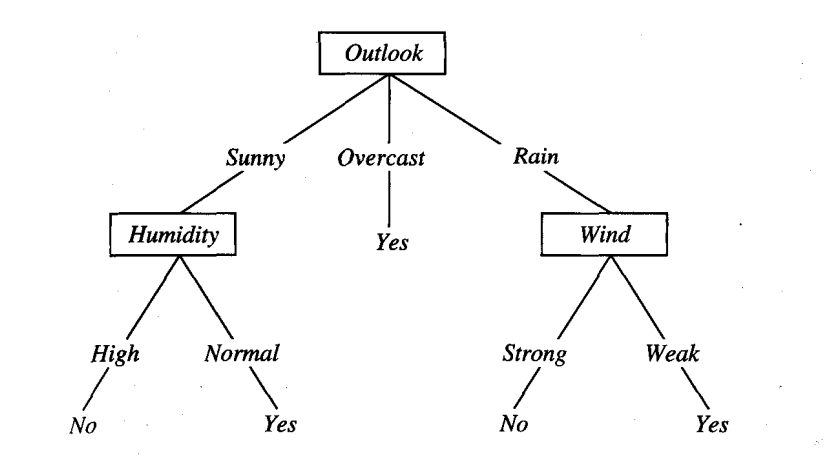
\includegraphics[width=\textwidth]{lemumu_koks_teorija}
	\caption{Lēmumu koka ilustrācija \cite{mitchell1997} }
	\label{fig:lemumu_koks_teorija}
\end{figure}

Piemērā \ref{fig:lemumu_koks_teorija} apskatām vienkāršu šāda koka reprezentāciju, kur veicam klasifikāciju par to vai šis ir piemērots laiks tenisa spēlei ārpus telpām. Ar ieejas datiem kā laikapstākļi (outlook) – saulaini (sunny), mitrums (humidity) – augsts (high), mēs virzītos pa mezgliem “Laikapstākļi”, “Mitrums” līdz lapas mezglam kurš klasificētu laiku kā nepiemērotu tenisa spēlei.

\subsubsection{Atbalsta vektoru mašīnas (SVM)}

Atbalsta vektora mašīnas \cite{supportvectornetworks} (\textit{support vector machines} jeb SVM) ir pārraudzītās mācīšanās algoritms kurš ir populārs tieši klasifikācijas problēmu risināšanā. Šis algoritms veic klasifikāciju konstruējot n-dimensiju hiperplakni kura optimāli ierobežo datus divās nošķirtās kategorijās. Lai vieglāk ilustrētu algoritma darbību, varam apskatīt divdimensiju piemēru.
\begin{figure}[H]
	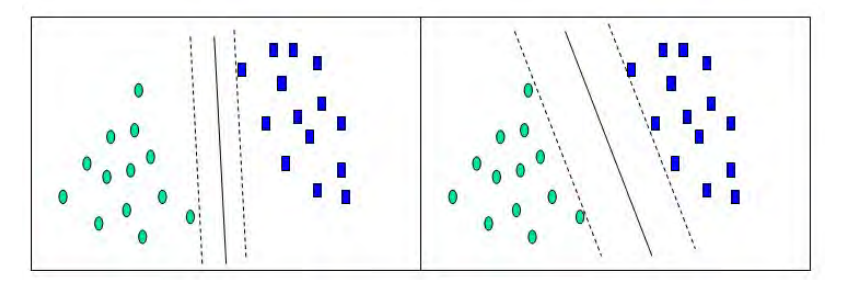
\includegraphics[width=\textwidth]{svm1}
	\caption{Atbalsta vektora mašīnas algoritma ilustrācija \cite{supportvectornetworks} }
	\label{fig:svm1}
\end{figure}
Šajā piemērā no \ref{fig:svm1} attēla - gadījumi ar vienu kategoriju atrodas pa kreisi (apzīmēti ar zaļiem apļiem) un ar otru kategoriju – pa labi (apzīmēti ar ziliem kvadrātiem). Atbalstu vektora mašīnas analīze mēģinās atrast 1-dimensijas hiperplakni (līniju) kura atdala datus balstoties uz kategoriju kurai tie pieder. Pastāv praktiski neierobežots līniju skaits, kas spētu veikt šādu nodalījumu, attēlā norādīti divi piemēri. Atliek gūt atbildi uz jautājumu – kura līnija ir labāka kategorizācijas veikšanai vispārīgā gadījumā. Raustītās līnijas, kuras zīmētas paralēli atdalošajai līnijai, iezīmē attālumu starp atdalošo līniju un tai tuvāko vektoru. Šo attālumu sauc par robežu (\textit{margin}). Vektori kas atrodas pie šīs robežas ir atbalsta vektori.
\begin{figure}[H]
	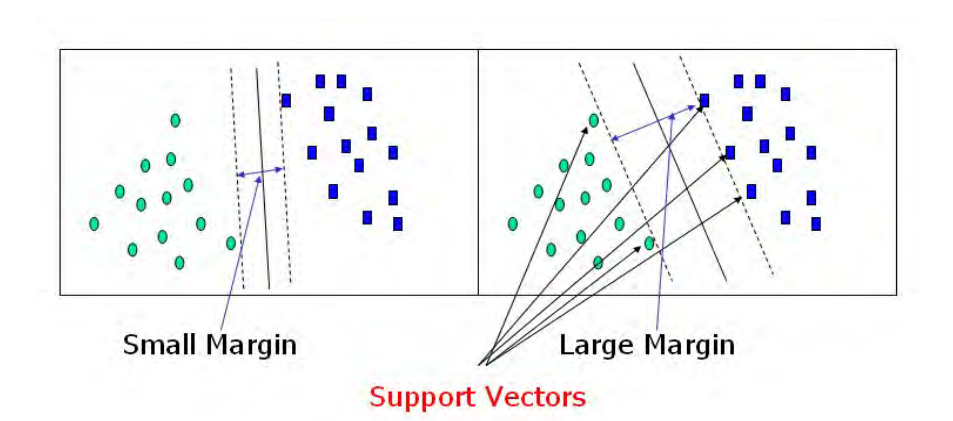
\includegraphics[width=\textwidth]{svm2}
	\caption{Robežas un atbalsta vektoru ilustrācija \cite{supportvectornetworks} }
	\label{fig:svm2}
\end{figure}
Atbalstu vektora mašīnas analīze atradīs līniju (vispārīgi – hiperplakni), kas novietota ar pēc iespējas lielāku robežu starp atbalsta vektoriem.

\section{Neironu tīkli}
Cilvēka smadzenes ir neironu tīkla arhitektūras iedvesmas avots. Cilvēka smadzeņu šūnas, ko sauc par neironiem, veido sarežģītu, savstarpēji cieši saistītu tīklu, kurā neironi sūta viens otram elektriskus signālus ar mērķi palīdzēt cilvēkiem apstrādāt informāciju. Līdzīgi mākslīgais neironu tīkls ir veidots no mākslīgiem neironiem, kas strādā kopā, lai atrisinātu problēmu \cite{AwsNeuralNetworks}. 

Sākumā jāapskata māklīgā neironu tīkla pamatvienība - neirons.
\begin{figure}[H]
	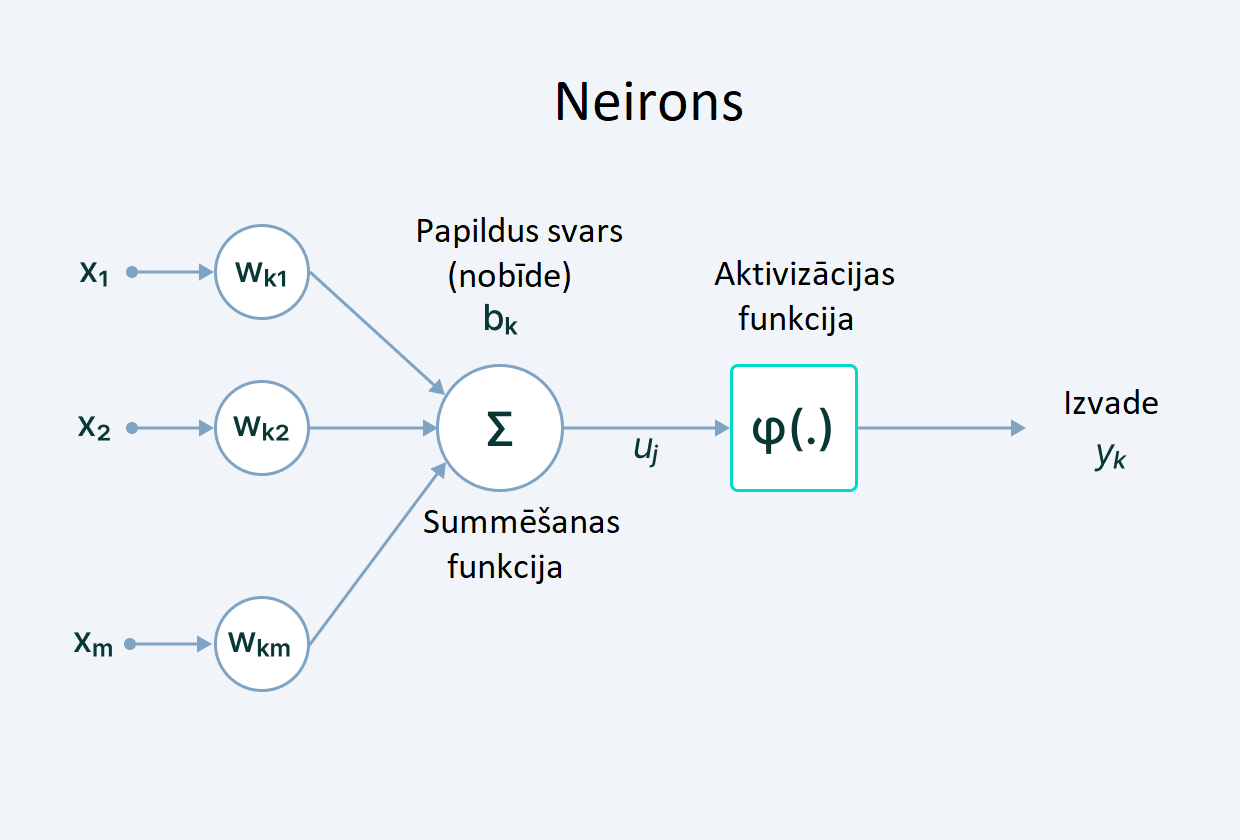
\includegraphics[width=\textwidth]{neirons}
	\caption{Mākslīgā neirona attēlojums}
	\label{fig:neirons}
\end{figure}

Kā redzams attēlā attēlā \ref{fig:neirons}, šī neirona uzbūvi raksturo tā pieci pamatelementi - ieejas signāls, svars, summēšanas funkcija, aktivizācijas funkcija un nobīde.

Ieejas signāls - tas ir neironā ienākošais signāls. Izcelsme tam var būt ārēja vai arī tas var būt cita neirona izejas signāls. Šādi ieejas signāli neironam var būt vairāki.

Svars - tā galvenā funkcija ir piešķirt lielāku nozīmi tiem ieejas signāliem, kas ir svarīgi pareizam problēmas risinājumam. Piemēram, negatīvs vārds ietekmētu noskaņojuma analīzes modeļa lēmumu vairāk nekā neitrālu vārdu pāris. Svara vērtības tiek noteiktas apmācības procesā.

Summēšanas funkcija - šīs funkcijas mērķis ir apvienot vairākus ieejas signālus un to svarus vienā vērtībā, ko tālāk padot aktivizācijas funkcijai.

Aktivizācijas funkcija - šī funkcija izrēķina aktivitātes stāvokli, kas bieži ir arī neirona izejas vērtība.	

Papildus svars (novirze) -  novirzes uzdevums ir sniegt svaru aktivizācijas funkcijas radītajai vērtībai. Tās loma ir līdzīga konstantes lomai lineārā funkcijā un, gluži kā svars, novirzes vērtība tiek noteikta apmācību procesā.

Kad vairāki neironi ir salikti kopā pēc kārtas, tie veido slāni. Vairākus slāņus apvienojot varam iegūt daudzslāņu neironu tīklu. Vispārēja daudzslāņu neironu tīkla arhitektūra, apskatīta \ref{fig:Artificial-neural-network-architecture}attēlā, aprakstāma kā savstarpēji savienoti mākslīgie neironi trijos vai vairāk slāņos.

\begin{figure}[H]
	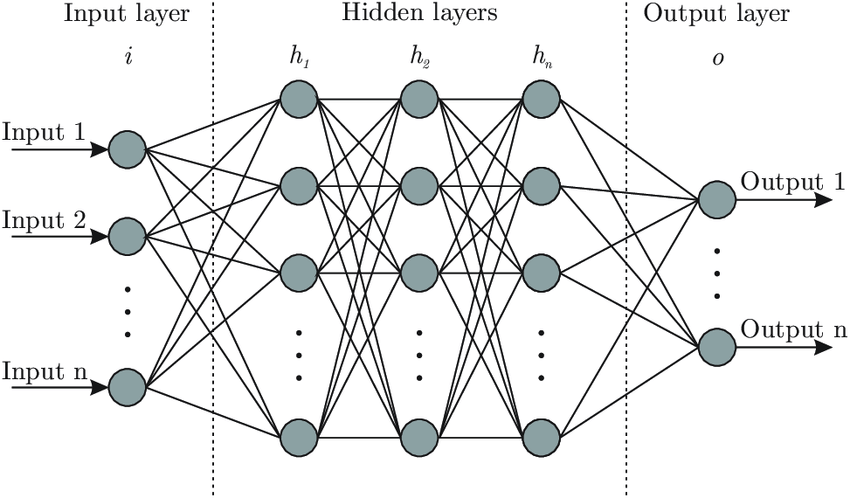
\includegraphics[width=\textwidth]{Artificial-neural-network-architecture}
	\caption{Mākslīgā neirona tīkla uzbūves vispārinājums \cite{artificialNeuralNetBre} }
	\label{fig:Artificial-neural-network-architecture}
\end{figure}

\textbf{Ievades slānis}

Informācija no ārpasaules caur ievades slāni nonāk mākslīgajā neironu tīklā. Ievades mezgli apstrādā datus, analizē vai klasificē tos un nodod tos nākamajam slānim.

\textbf{Slēptie slāņi}

Slēptie slāņi izmanto ievadi no ievades slāņa vai citiem slēptiem slāņiem. Mākslīgajiem neironu tīkliem var būt liels skaits slēpto slāņu. Katrs slēptais slānis analizē iepriekšējā slāņa izvadi, apstrādā to tālāk un nodod nākamajam slānim.

\textbf{Izvades slānis}

Izvades slānis sniedz visu mākslīgā neironu tīkla veiktās datu apstrādes gala rezultātu. Tam var būt viens vai vairāki mezgli. Piemēram, ja mums ir bināra (jā/nē) klasifikācijas problēma, izvades slānim būs viens izvades mezgls, kas dos rezultātu 1 vai 0. Tomēr, ja mums ir vairāku klašu klasifikācijas problēma, izvades slānis var sastāvēt no vairāk nekā viena izvades mezgla.

\subsection{Konvolūcijas neironu tīkli}
Konvolūcijas neironu tīklu sākotnējais mērķis ir bijis datorredzes problēmu risināšana ar dziļās mašīnmācīšanās palīdzību, tomēr laika gaitā šāda neironu tīklu arhitektūra ir guvusi plašu pielietojumu arī dabīgās valodas apstrādē. Kim Yoon 2014. gadā ir pierādījis ka teikumu klasifikācijā tieši konvolūcijas neironu tīklu spēj sniegt labākus rezultātus par citiem neironu tīklu modeļiem \cite{kimYoonCNN}. Cits populārs neironu tīkla veids valodas apstrādē ir rekurentie neironu tīkli ar ilgtermiņa atmiņu (LSTM balstīti modeļi) - šāda pieeja ļauj gūt labus rezultātus apstrādē kur liela nozīme ir vārdu secībai un atkarībai no citiem apkārt esošiem vārdiem, piemēram, mašīntulkošanā. Teksta klasifikācijā šādas valodas izpratnes nozīme nav tik izteikta, piemēram, Ņujorkas Universitātes pētnieku salīdzinājums starp dažādiem modeļiem teksta klasifikācijā \cite{zhang2015characterlevel}, pielietojot tos uz dažādām datu kopām, skatāms \ref{appendix:zhang_models} pielikumā. Kā redzams no šiem datiem, labākos rezultātus sasniedz klasiski modeļi ar loģistisko regresiju un KNT modeļi (atkarībā no datu kopas), LSTM modeļiem neuzrādot labākus veiktspējas rādītājus nevienā no apskatītajām datu kopām. Savukārt Mathieu Cliche pētījumā par sentimenta analīzi uz dažādu gadu Twitter datu kopām \cite{cliche-2017-bb}, salīdzinot KNT un LSTM modeļus, iegūtie akurātuma rezultāti dažu gadu datu kopās (skatīt tabulu \ref{appendix:twitter_models} pielikumā) sasniedz vienādus rezultātus (2013., 2014. un  2016. gada dati), savukārt 2015. gada datiem labāko rezultātu uzrādot KNT modeļiem. Balstoties uz augstākminētajiem salīdzinājumiem, arī autors izvēlējies vispirms pārbaudīt KNT arhitektūru un tās spēju veiksmīgi klasificēt latviešu valodas ziņu rakstus. Sākumā tiek apskatīti pamatslāņi, kurus apvienojot iespējams veidot konvolūcijas neironu tīklus.

\subsubsection{Iegulšanas slānis}
Neironu tīklā iegulšanas slānis pārvērš ievades vārdus vektoru attēlojumā, veidojot vārdlietojuma kartējumu (jau iepriekš apskatītu pie vektorizācijas pieejām). Šis ir svarīgs solis, lai modelis varētu efektīvi apstrādāt un saprast teksta datus, it īpaši vārdu kontekstu. Vārdi ar līdzīgām nozīmēm tiek kartēti kā līdzīgi vektori, ļaujot izprast vārdu saistības un teikuma uzbūves sakarības. Šie vektori ir apmācāmi parametri, respektīvi, apmācības laikā tiek modificēti to svari, ļaujot neironu tīklam apgūt vispiemērotāko vārdu attēlojumu konkrētajam uzdevumam.

\subsubsection{Konvolūcijas slānis}
Konvolūcijas darbības princips ir filtru pielietošana, secīgi ejot cauri ievadei un meklējot dažādas pazīmes. Atkarībā no apskatāmās problēmas šie filtri var ieņemt dažādas  formas – pielietojot konvolūciju uz attēliem parasti tiks pielietoti trīs dimensiju filtri. Teksta apstrādes gadījumā savukārt tiek lietoti viendimensionāli filtri ar noteiktu platumu, ko parasti sauc par kodola (\textit{kernel}) izmēru. Piemēram, kodola izmērs kā 3 nozīmētu to, ka vienlaikus filtrs apskatīs trīs secīgus vārdus. Filtrs tiek pārvietots pār ievades virkni un kovolūcija tiek veikta veicot skalāro reizinājumu starp filtru un apskatīto virknes posmu. Rezultātā katrā posmā tiek iegūta vērtība, kas norāda meklētās pazīmes klātbūtni. Konvolūcijas slānis parasti satur vairākus šādus filtrus un katrs filtrs ir atbildīgs par dažādu pazīmju pārbaudi ievades datos. Apmācības laikā neironu tīkls nosaka optimālos svarus katram no šiem filtriem, norādot dažādu pazīmju nozīmi pareizas izvades iegūšanai.

\begin{figure}[H]
	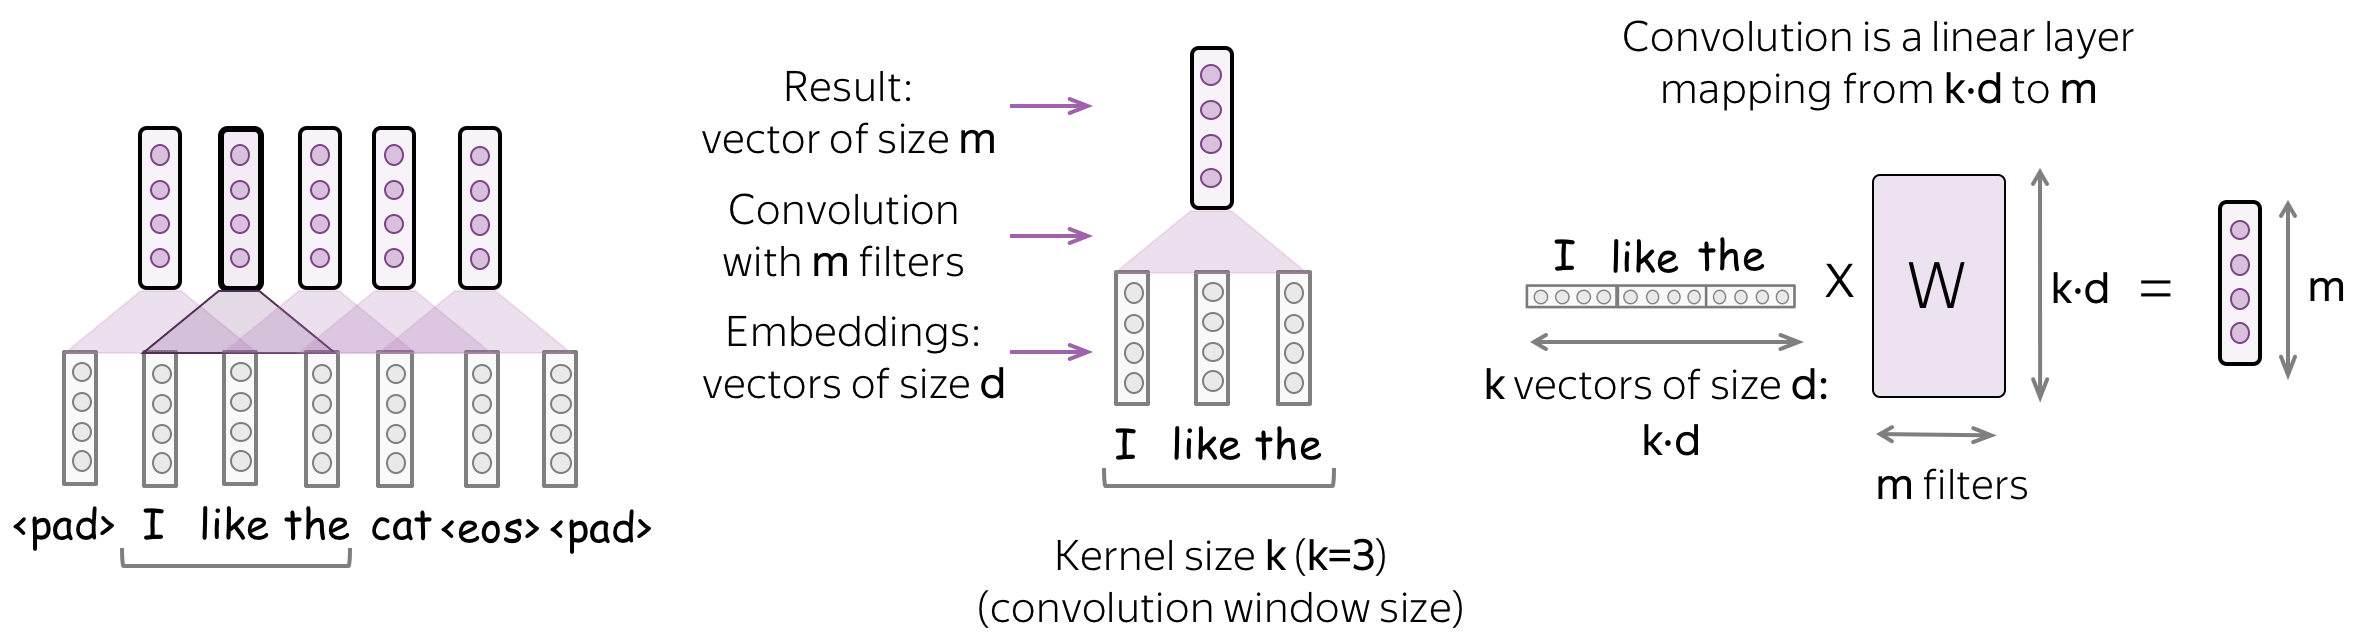
\includegraphics[width=\textwidth]{convolution_linear_layer-min}
	\caption{Konvolūcijas slānis \cite{TextCNNLena}}
	\label{fig:convolution_linear_layer}
\end{figure}

\subsubsection{Apvienošanas slānis}

Apvienošanas slānis veic ievades datu samazināšanas procedūru, atmetot mazsvarīgāku informāciju un saglabājot svarīgākos datu punktus, rezultātā nodrošinot efektīvāku tīkla darbību (mazāks apstrādājamo parametru skaits). Slāņa darbības principu apskatam iekš \ref{fig:pooling_vs_global} attēla.

\begin{figure}[H]
	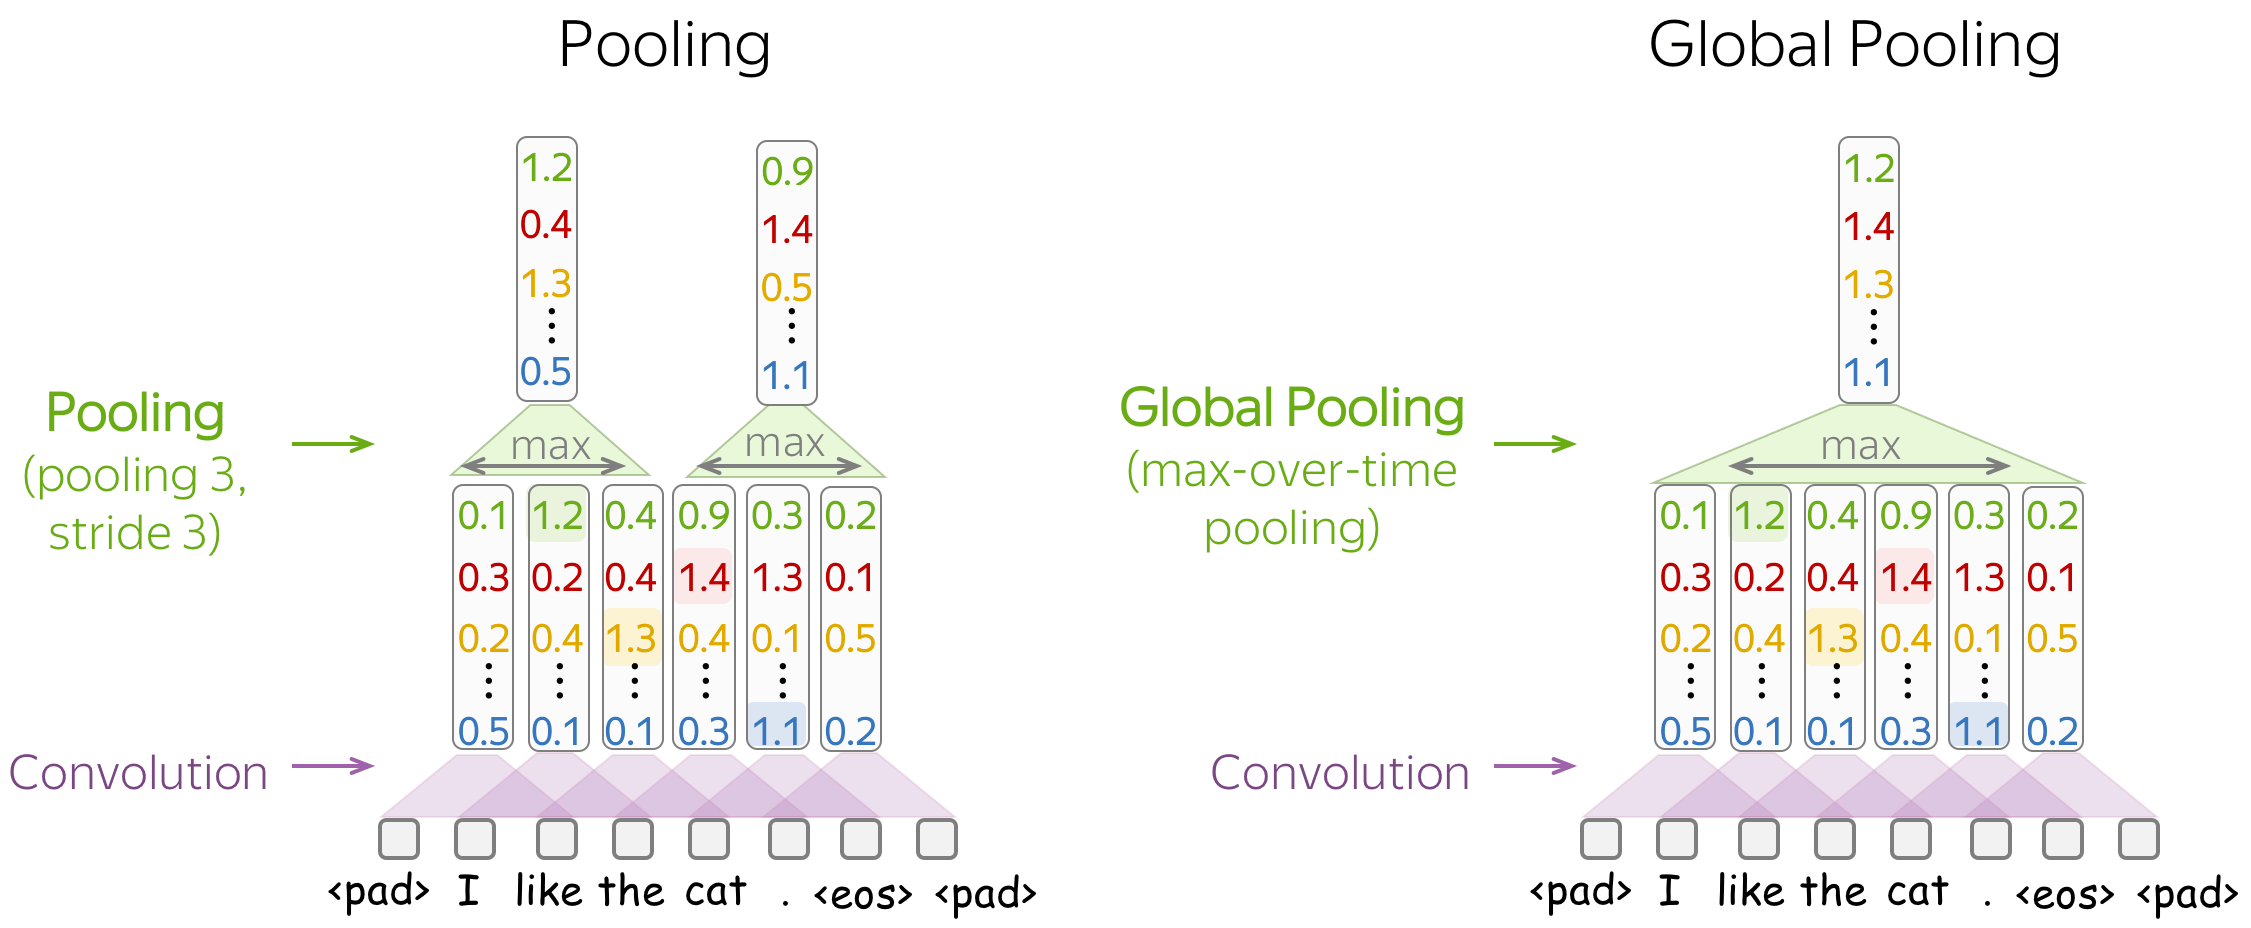
\includegraphics[width=\textwidth]{pooling_vs_global-min}
	\caption{Apvienošanas slānis \cite{TextCNNLena}}
	\label{fig:pooling_vs_global}
\end{figure}

Galvenā ideja ar maksimālo apvienošanu ir atrast lielāko vērtību katrā dimensijā jeb atrast lielāko vērtību katrai pazīmei, rezultātā iegūstot vektoru, kurš norāda kādas pazīmes apskatāmajā ievades tekstā ir atrastas. Alternatīvi var izmantot arī vidējās vērtības apvienošanu, kur gala vektora vērtība tiek veidota nevis no maksimālās, bet vidējās vērtības apskatāmajā dimensijā. Kā redzams \ref{fig:pooling_vs_global} attēlā - šādas apvienošanas operācijas varam veikt ar noteiktu soļa izmēru (\textit{stride}) vai pielietojot uz visu ievades virkni. 

\subsubsection{Atmešanas slānis}
Lai izvairītos no pārmērīgas pielāgošanas apmācības laikā bieži tiek lietots arī atmešanas slānis (\textit{dropout}). Slāņa princips ir nejaušības kārtā “atmest” daļu no iegūtajām vērtībām jeb konkrētāk - iestatīt daļu no tām kā 0, kas palīdz vispārināt modeli un labāk reaģēt uz neredzētiem ievades datiem. Šādam slānim parasti arī definējam atmešanas rādītāju (\textit{dropout rate}), kas norāda kādu daļu no neironiem mēs atmetam apmācību laikā, vērtība visbiežāk tiek izvēlēta robežās no 0.2 līdz 0.5.

\subsubsection{Pilnīgi savienotais slānis}
Konvolūcijas neironu tīklā kā pēdējais slānis ir pilnīgi savienotais slānis, kas apvieno tīkla iepriekšējo slāņu rezultātus, lai veiktu minējumu par ievades piederību kategorizācijas klasēm. Pārsvarā šajā slānī izmanto softmax aktivizācijas funkciju ar kuras palīdzību pārvēršam slānim padotās skaitliskās vērības par varbūtības vērtībām katrai klasei (robežās no 0 līdz 1) un kur visu klašu varbūtību summa būs kā 1. Ja dots ievades vektors ar rezultātiem katrai klasei kā \(z = (z_1, z_2, ..., z_k)\), tad softmax funkciju i-tajam elementam varam definēt kā:
\begin{equation}
softmax(z)_i = \frac{e^{z_i}}{\sum_{j=1}^{k} e^{z_j}}
\end{equation}

\noindent kur:
\begin{itemize}
\item \(e\) ir Eilera skaitlis.
\item \(z_i\) ir skaitliskais rezultāts \(i\)-tajai klasei.
\item Dalītājs ir eksponentfunkciju summa visiem skaitliskajiem rezultātiem.
\end{itemize}

Ilustrējot ar piemēru, ja dots izvades slānis ar vektoru \(z = (2.0, 1.0, 0.1)\) trīs klašu klasifikācijai, iegūtās varbūtības katrai klasei būtu:

\[ \text{softmax}(z)_1 = \frac{e^{2.0}}{e^{2.0} + e^{1.0} + e^{0.1}} = 0.65900114\]

\[ \text{softmax}(z)_2 = \frac{e^{1.0}}{e^{2.0} + e^{1.0} + e^{0.1}} = 0.24243297\]

\[ \text{softmax}(z)_3 = \frac{e^{0.1}}{e^{2.0} + e^{1.0} + e^{0.1}} = 0.09856589\]

Klasi ar lielāko varbūtību pieņemam kā gala minējumu. Slāņa darbība un mijiedarbība ar citiem slāņiem apskatāma \ref{fig:model_cnn_basic} attēlā.

\begin{figure}[H]
	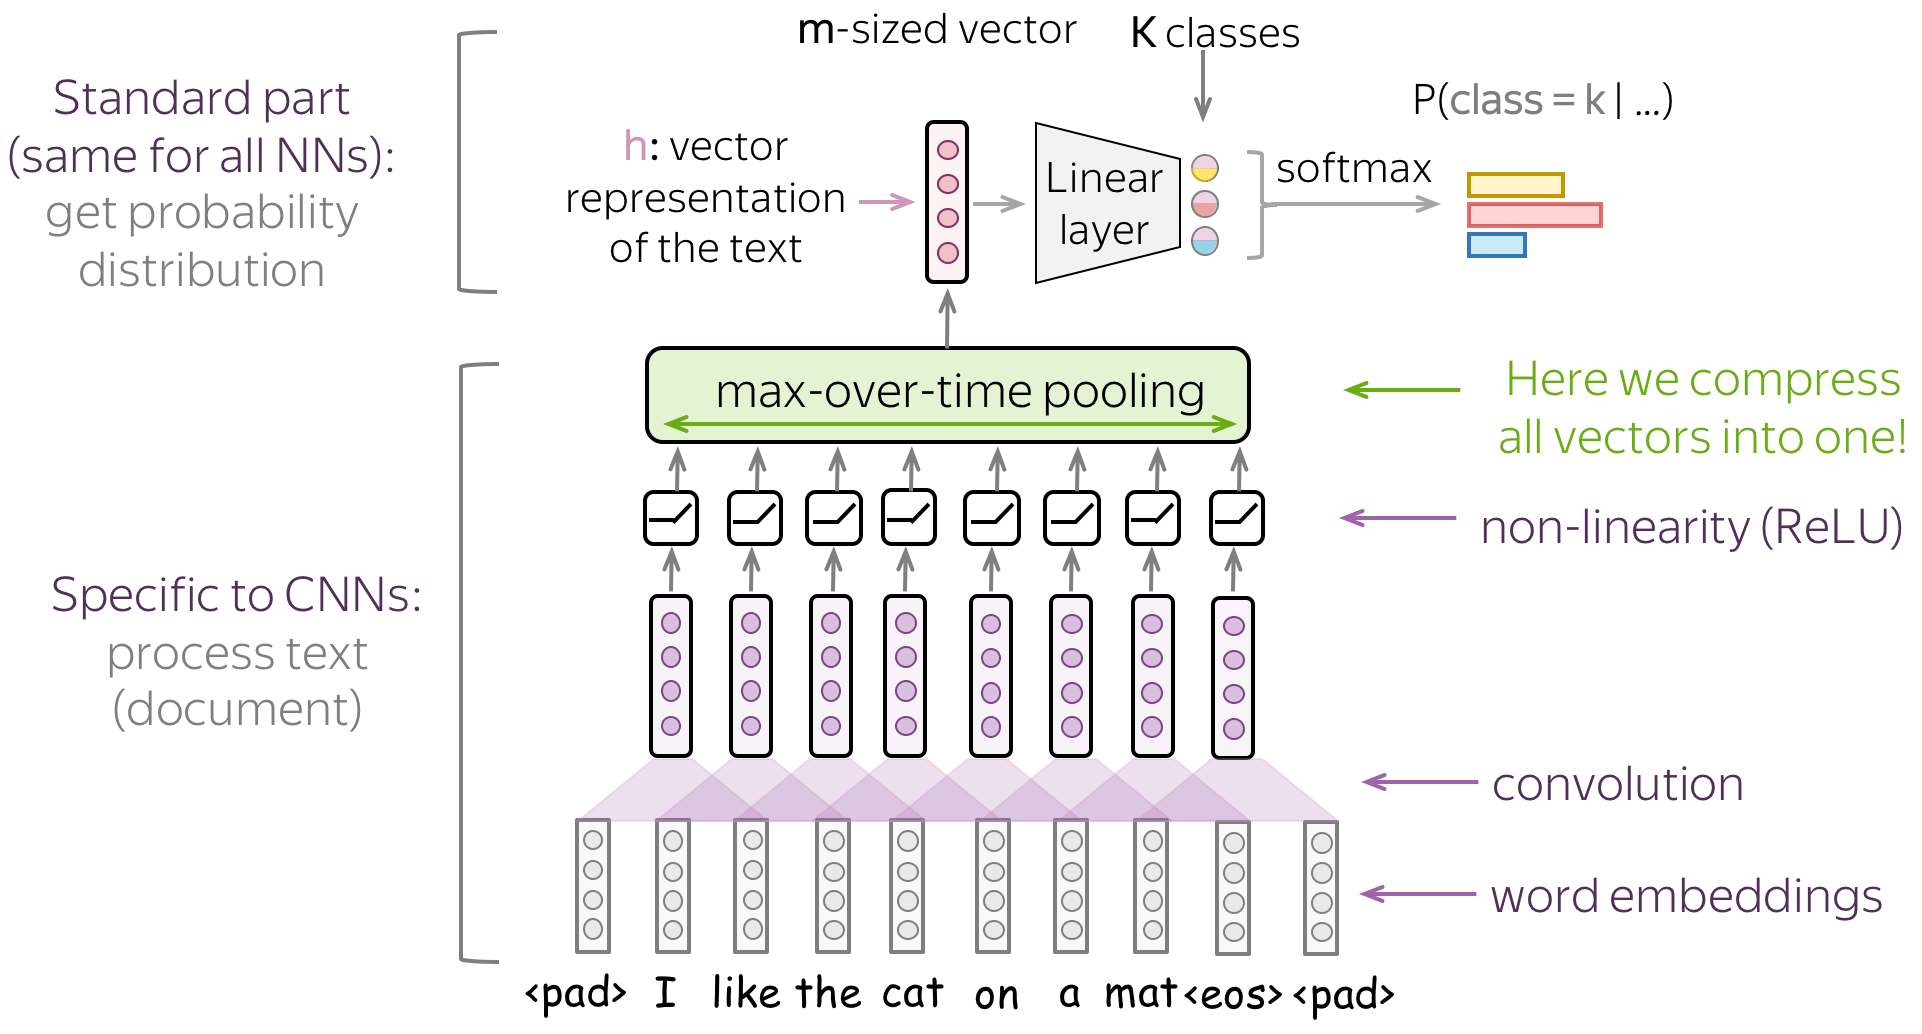
\includegraphics[width=\textwidth]{model_cnn_basic-min}
	\caption{Konvolūcijas neironu tīkls tekstu klasifikācijai \cite{TextCNNLena}}
	\label{fig:model_cnn_basic}
\end{figure}

Standarta arhitektūrai iespējams arī veikt dažādus uzlabojumus, viena no literatūrā biežāk minētajām pieejām, ko piedāvā Kim Yoon \cite{kimYoonCNN}, ir pielietot paralēli vairākus konvolūcijas un apvienošanas slāņus ar dažādiem filtra izmēriem (pētījumā filtri izvēlēti ar izmēriem kā 2,3 un 4), vēlāk šos slāņus apvienojot pirms padošanas tālāk.

\begin{figure}[H]
	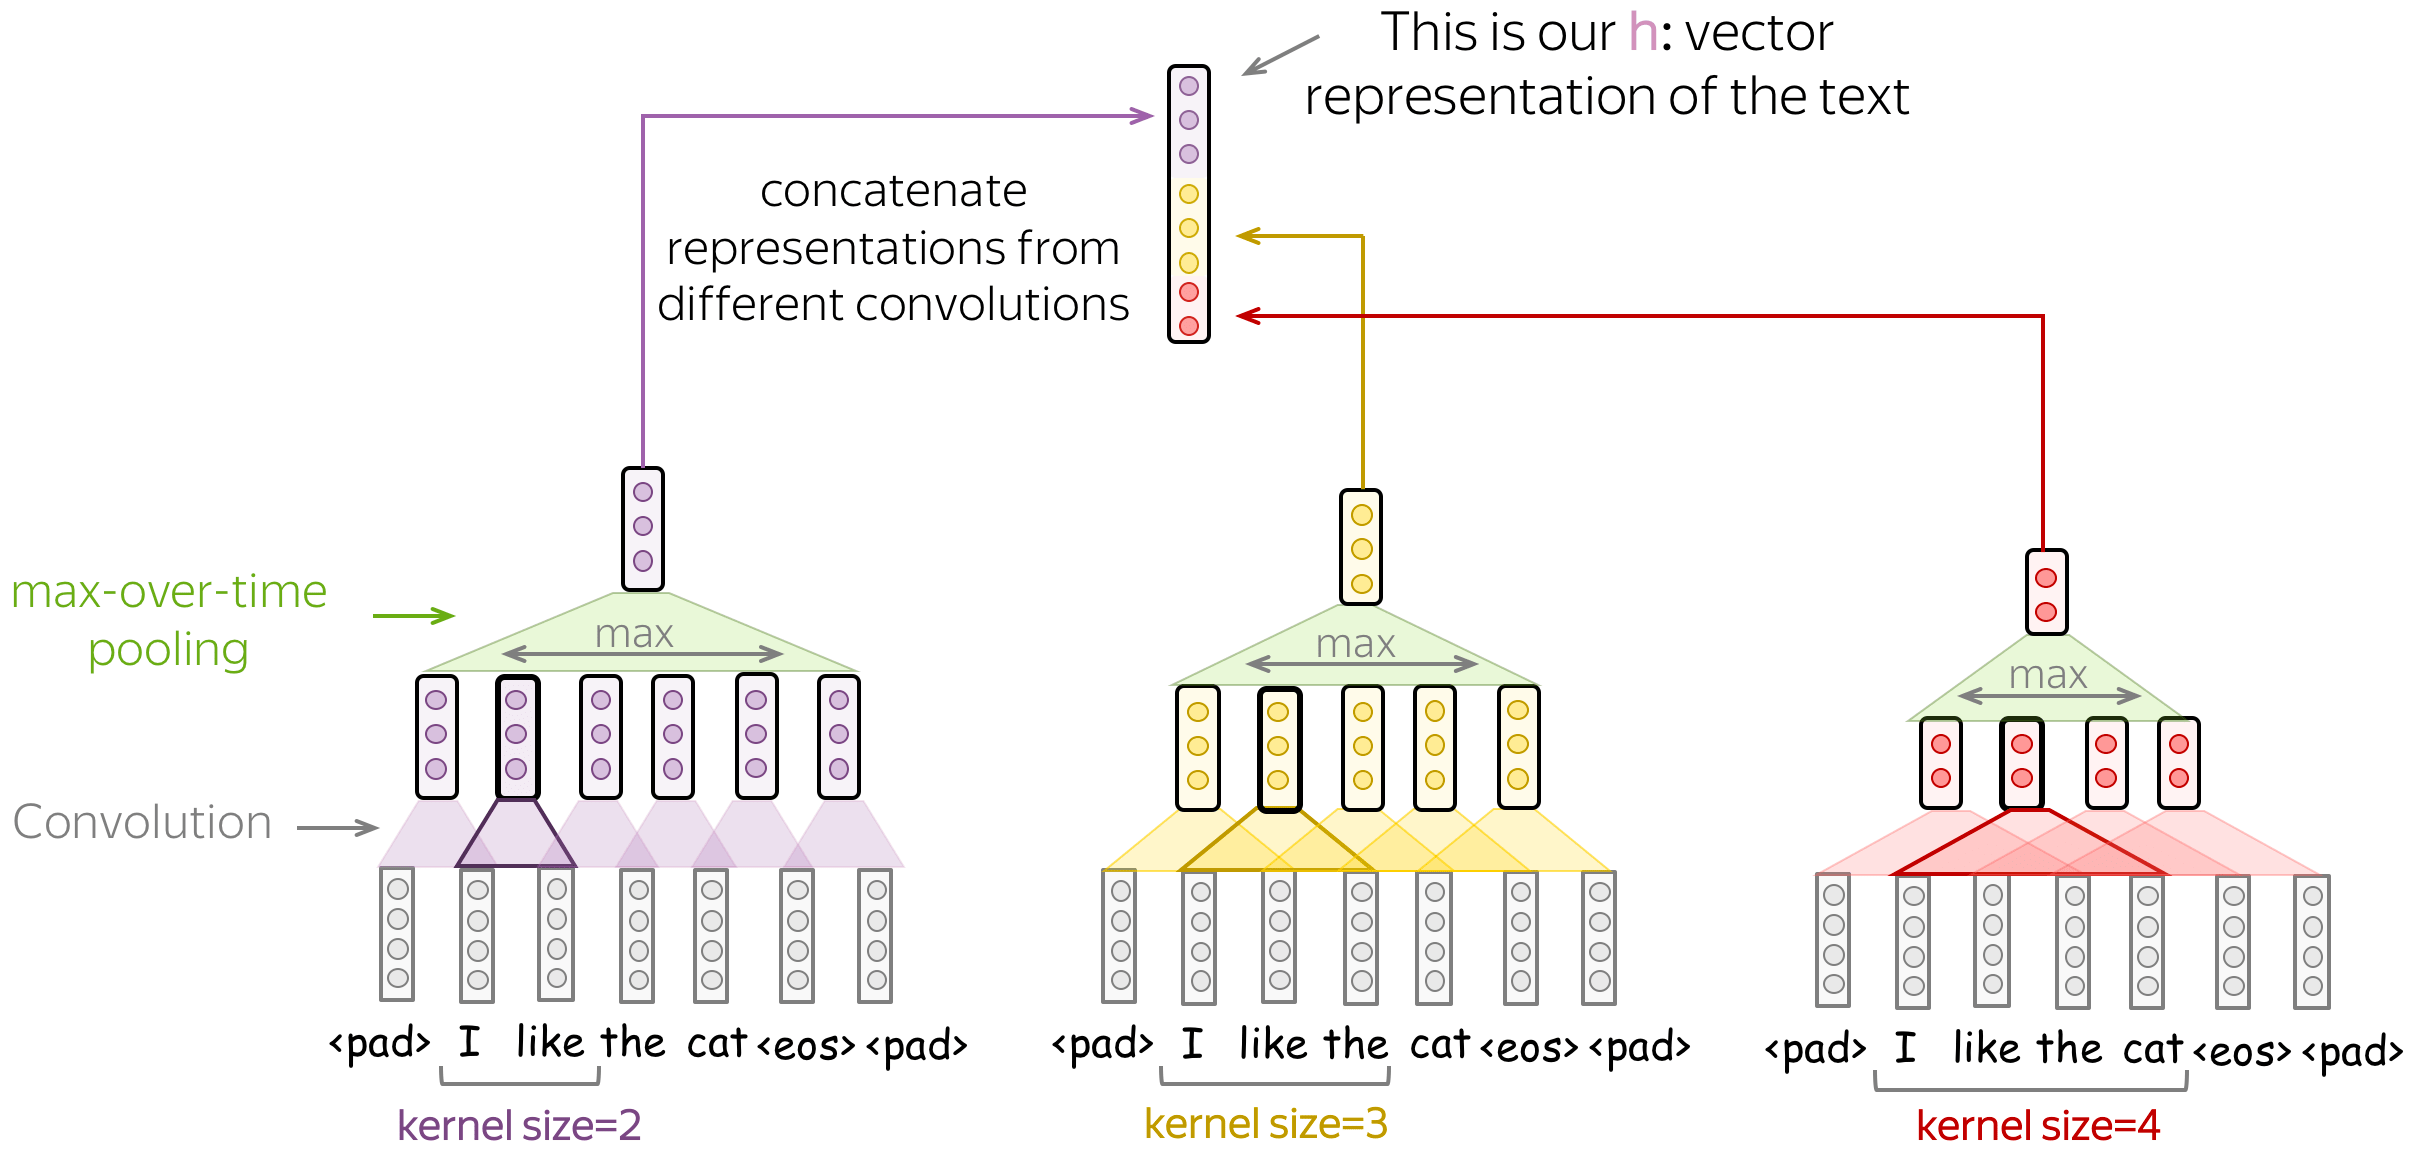
\includegraphics[width=\textwidth]{KNT_konkatenacija}
	\caption{Arhitektūra ar dažādu izmēru konvolūcijas slāņiem \cite{TextCNNLena}}
	\label{fig:KNT_konkatenacija}
\end{figure}

\subsection{Rekurentie neironu tīkli}
Rekurentie neironu tīkli (RNT) ir neironu tīkla veids, kas palīdz apstrādāt secīgus datus, piemēram, tekstus, ņemot vērā to secību un atkarības starp datiem. Šie tīkli satur rekurentus savienojumus neironu tīklā ar kuru palīdzību iespējams saglabāt slēpto stāvokli ar informāciju no iepriekšējiem apstrādes soļiem.

\begin{figure}[H]
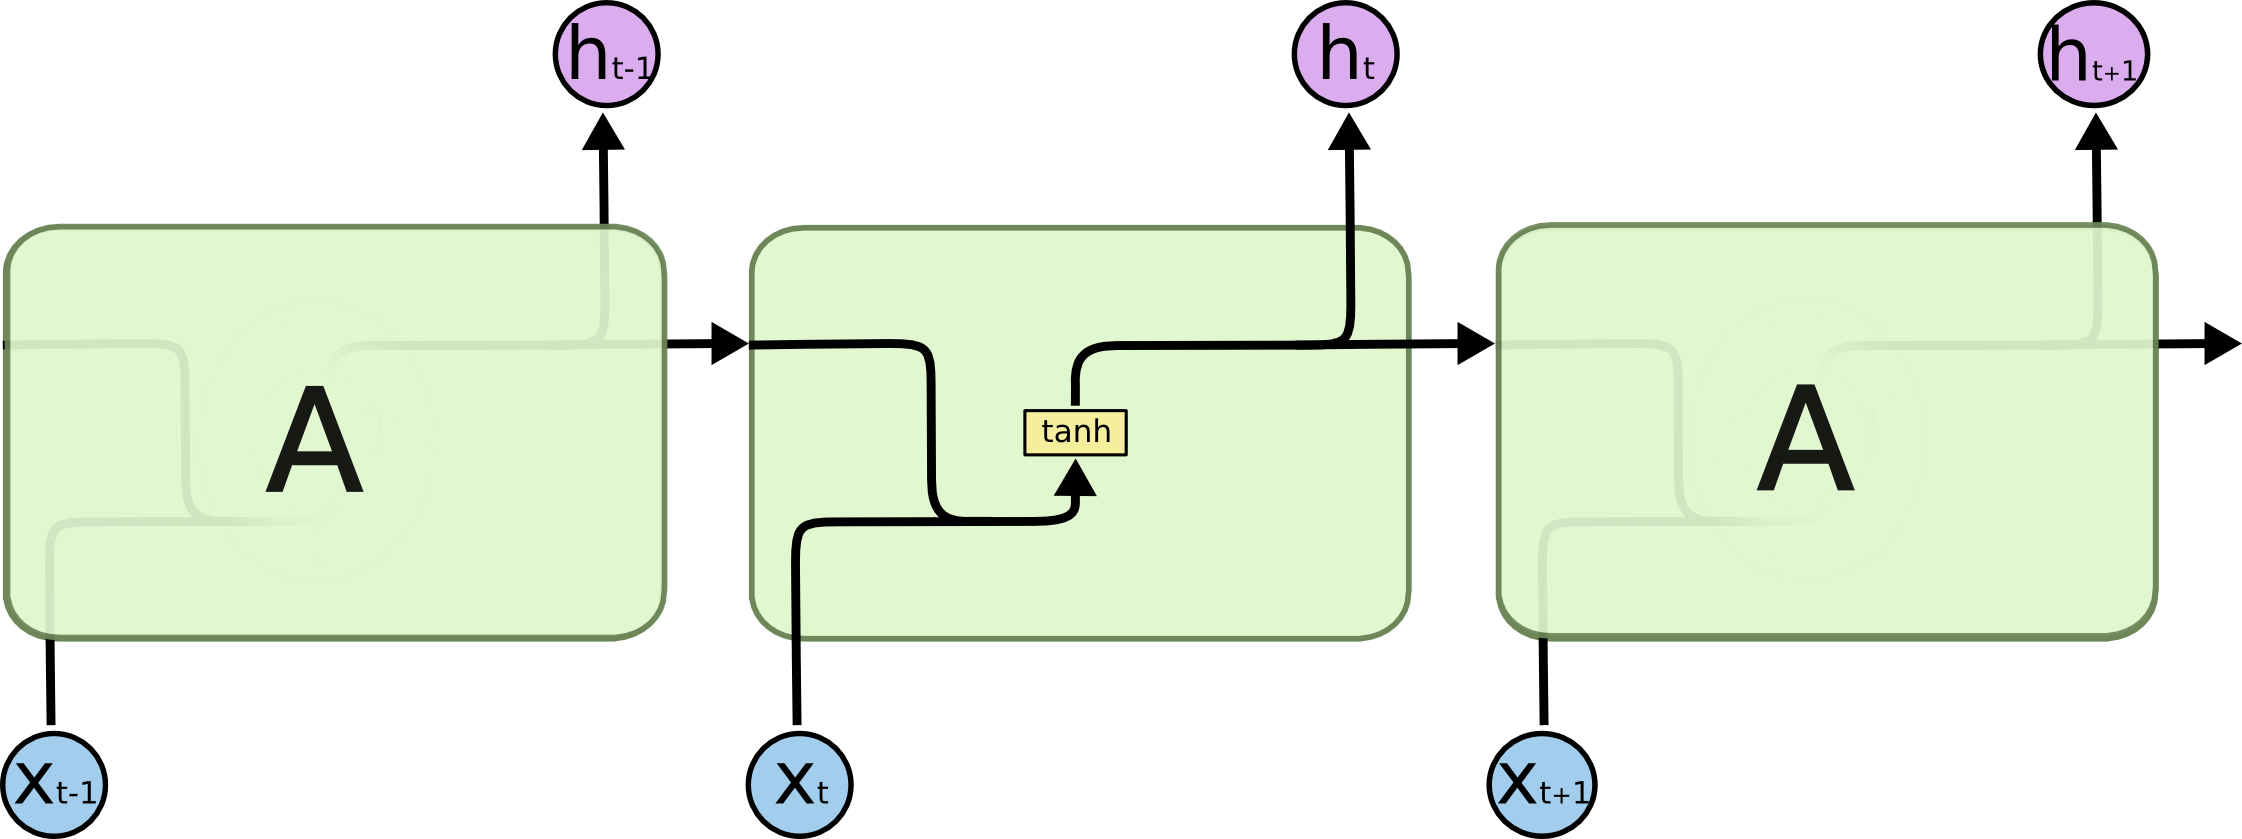
\includegraphics[width=\textwidth]{LSTM-SimpleRNN}
\caption{RNT ilustrācija \cite{ChristopherOlahLSTM}}
\label{fig:LSTM-SimpleRNN}
\end{figure}

\subsubsection{Gradientu zušana}
Neironu tīklos gradienti kalpo kā indikatori svara korekcijai, samazinot atšķirību starp prognozētajiem un faktiskajiem rezultātiem. Tomēr gradienti bieži kļūst aizvien mazāki, virzoties caur tīkla slāņiem, potenciāli izraisot mācīšanās palēnināšanos vai pat apstāšanos sākotnējos slāņos. Šo parādību sauc par izzūdošā gradienta problēmu. Rekurento neironu tīklu gadījumā šī parādības a rodas no rekurentajiem savienojumiem un gradientu vērtībām pēc daudziem soļiem, respektīvi, katrā laika posmā RNT šūna izmanto gan pašreizējo ievadi, gan slēpto stāvokli no iepriekšējā laika posma, lai aprēķinātu jaunu slēpto stāvokli un izveidotu izvadi. Šī atkarība no iepriekšējiem laika posmiem izraisa gradienta izplatīšanos, izmantojot atkārtotu savienojumu ķēdi. Veicot aprēķinus par vairākiem iepriekšējiem soļiem – šo sākotnējo soļu gradienti var kļūt ļoti mazi, jo katrā laika posmā tiek atkārtoti aprēķināti gradienti. Tie var samazināties līdz stāvoklim, kur tie faktiski ir ar nulles vērtību. Rezultātā secības agrākie laika soļi apmācības laikā saņem ļoti vājus gradienta signālus. Turklāt to atbilstošie svari tiek atjaunināti lēni vai netiek atjaunināti vispār. Tas noved pie svarīgas informācijas zaudēšanas un lēnas mācīšanās konverģences.

\subsubsection{LSTM}
LSTM tika izstrādāts lai mēģinātu risināt izzūdošā gradienta problēmu. Lai to izdarītu, LSTM izmanto vārteju mehānismus, lai kontrolētu informācijas plūsmu un gradientus. Tas palīdz novērst izzūdošu gradienta problēmu un ļauj tīklam mācīties un saglabāt informāciju garākās virknēs.

LSTM pamatā ir šūnas stāvoklis, kas tiek nodots no šūnas ievades uz izvadi, veidojot sava veida ilgtermiņa atmiņu (ilustrēts \ref{fig:LSTM-chain} attēlā). Pamatā ir 3 vārtejas – aizmiršanas vārti, ieejas vārti, izvades vārti. Informācija plūst pa visu ķēdi tikai ar nelielām lineārām darbībām caur trim vārtiem, kas nosaka informācijas plūsmu un to kāda informācija tiek saglabāta vai ignorēta.

\begin{figure}[H]
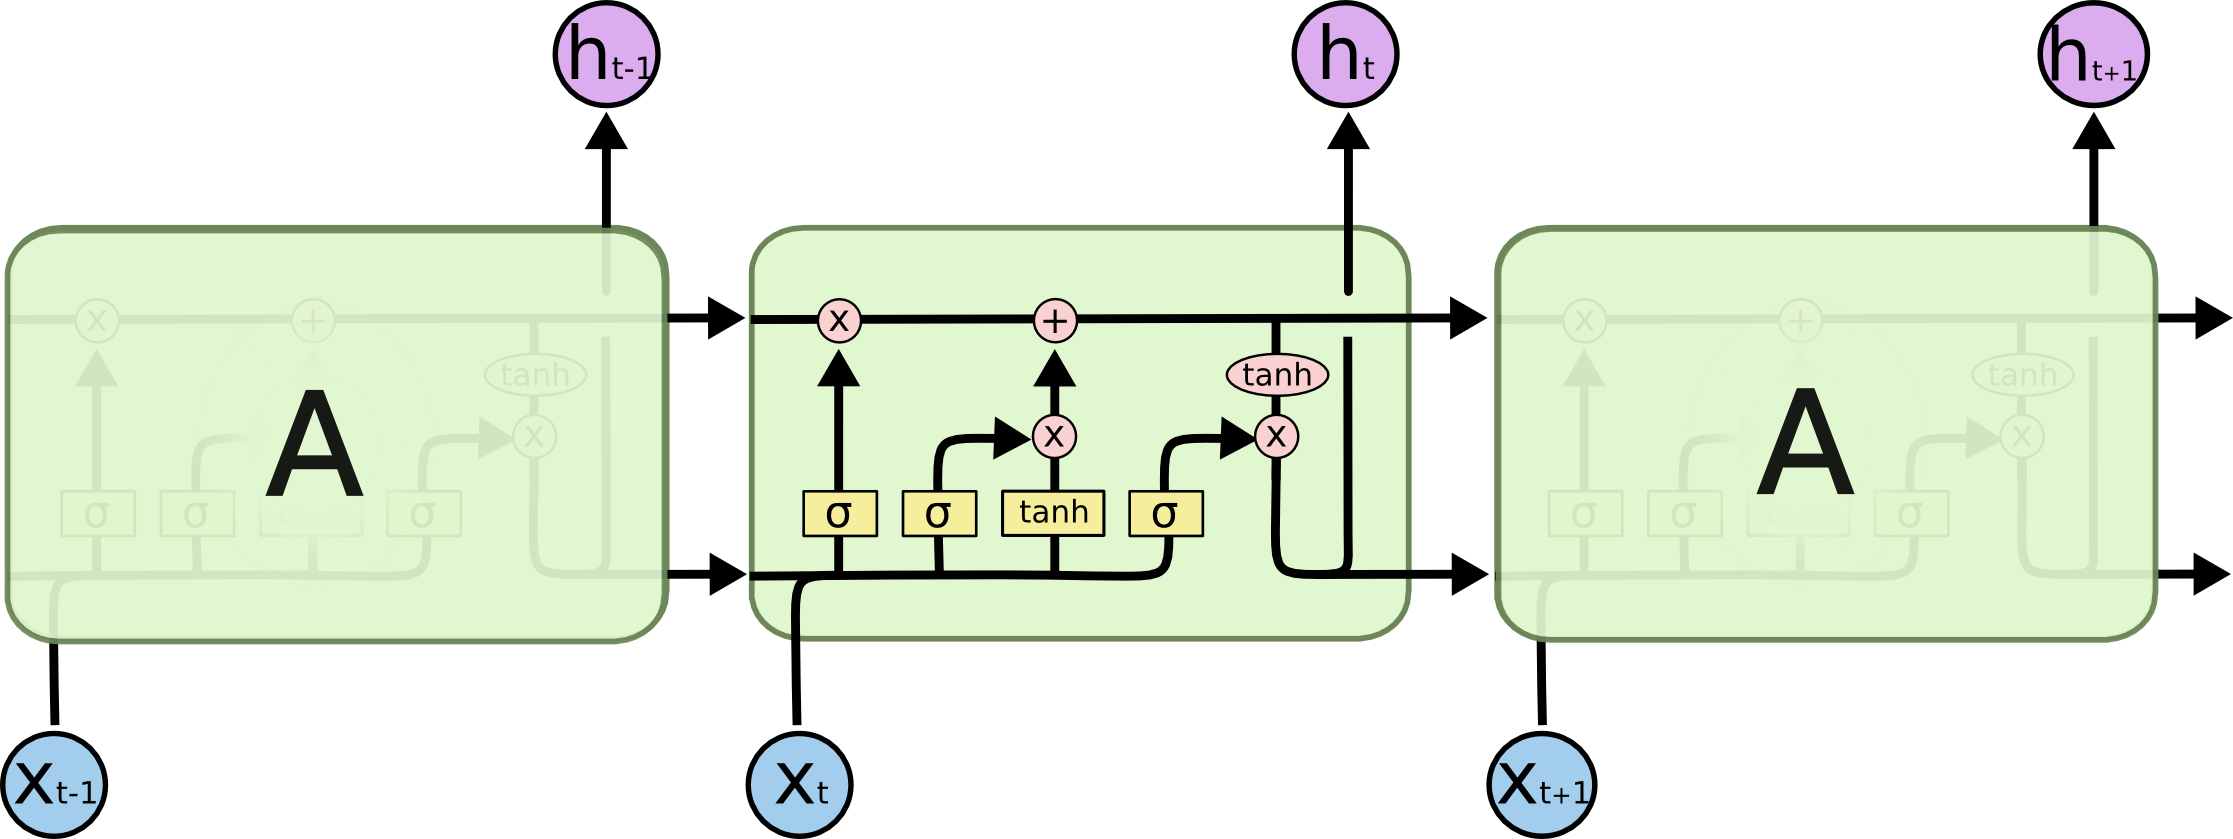
\includegraphics[width=\textwidth]{LSTM-chain}
\caption{LSTM ilustrācija \cite{ChristopherOlahLSTM}}
\label{fig:LSTM-chain}
\end{figure}

Aizmiršanas vārti izlemj, cik daudz no ilgtermiņa atmiņas jeb šūnas stāvokļa jāpārnes no iepriekšējā šūnas stāvokļa uz nākošo . Šim nolūkam tiek izmantota sigmoīda funkcija, kas norāda šūnas stāvokļa nozīmi. Izvade \(f_t\) svārstās no 0 līdz 1 un norāda, cik daudz informācijas tiek saglabāts, t.i., 0 - nesaglabāt informāciju un 1 - saglabāt visu informāciju par šūnas stāvokli. Aizmiršanas vārtus raksturo formula

\begin{equation}
f_t = \sigma \left( W_{f, x} x_t + W_{f, h} h_{t-1} + b_f \right)
\end{equation}

Kur:

- \( \sigma \) ir sigmoīda aktivācijas funkcija.

- \( W_{f, x} \) ir ievades svaru matrica  \( x_t \) laika solī \( t \).

- \( x_t \) ir ievades vektors laika solī  \( t \).

- \( W_{f, h} \)  ir slēptā stāvokļa svara matrica \( h_{t-1} \) no iepriekšējā laika soļa.

- \( h_{t-1} \) ir slēptais stāvoklis no iepriekšējā laika soļa.

- \( b_f \) ir aizmiršanas vārtu novirzes vērtība.

Ievades vārti izlemj, kura informācija jāpievieno šūnas stāvoklim un tādējādi arī ilgtermiņa atmiņai. Izvade \(i_t\) svārstās no 0 līdz 1 un norāda, cik daudz informācijas tiek pievienots, t.i., 0 - nepievienot jaunu informāciju un 1 - pievienot visu jauno informāciju. Šo vārteju raksturo zemāk minētā formula.
\begin{equation}
i_t = \sigma \left( W_{i, x} x_t + W_{i, h} h_{t-1} + b_i \right)
\end{equation}

Izvades vārti izlemj kuras šūnas stāvokļa daļas veido izvadi. Tādējādi izejas vārti ir atbildīgi par īstermiņa atmiņu. Izvade \(o_t\)  svārstās no 0 līdz 1 un norāda, cik daudz no šūnas stāvokļa tiek izvadīts, t.i., 0 - neizvadīt neko par šūnas stāvokli un 1 - izvadīt visušūnas stāvokli. Vārteju raksturo sekojoša formula.
\begin{equation}
o_t = \sigma \left( W_{o,x} x_t + W_{o,h} h_{t-1} + b_o \right)
\end{equation}

Kā redzams, visus trīs vārtus attēlo viena un tā pati funkcija. Atšķiras tikai svari un novirzes. Šūnas stāvoklis tiek atjaunināts, izmantojot aizmiršanas vārtus un ievades vārtus.
\begin{equation}
c_t = (f_t \cdot c_{t-1}) + (i_t \cdot \tanh(h_{t-1}))
\end{equation}

Pašreizējā laika soļa slēpto stāvokli \(h_t\) nosaka izejas vārti un tanh funkcija, kas ierobežo šūnas stāvokli no -1 līdz 1.
\begin{equation}
h_t = o_t \cdot \tanh(c_t)
\end{equation}

\subsubsection{Divvirzienu LSTM}
Divvirzienu LSTM jeb BiLSTM ir LSTM arhitektūras variants, kas sastāv no diviem atsevišķiem LSTM slāņiem - viens slānis apstrādā ievades datus secīgi, bet otrs apstrādā ievadi apgrieztā secībā. Šo divu LSTM slāņu izejas tiek apvienotas katrā laika solī, iegūstot galīgo izejas rezultātu. Šāda arhitektūra ilustrēta \ref{fig:BiLSTM} attēlā.

\begin{figure}[H]
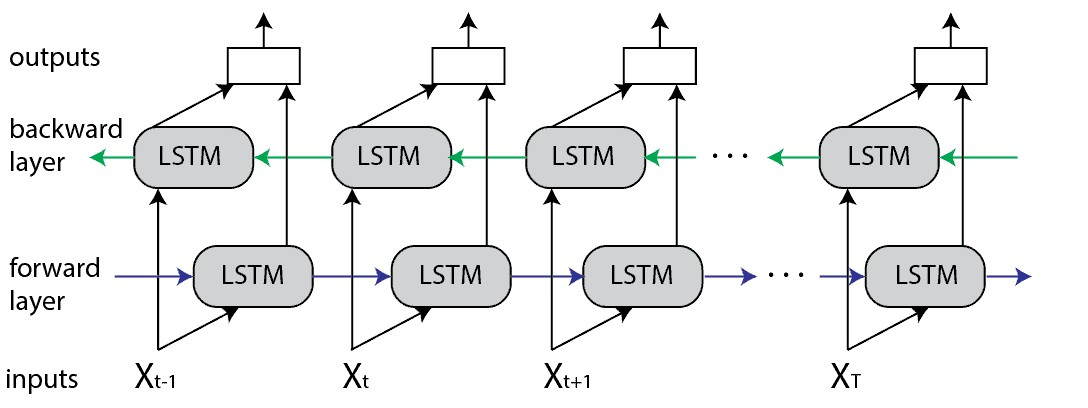
\includegraphics[width=\textwidth]{BiLSTM-visualization}
\caption{Divvirzienu LSTM ilustrācija \cite{BaeldungBiLSTM}}
\label{fig:BiLSTM}
\end{figure}

Galvenā šādas pieejas priekšrocība ir plašāka konteksta un vārdu sasvstarpējo atkarību izpratne, apskatot vārdus gan pēc, gan pirms konkrētā fragmenta.

\subsection{Transformatori un lielie valodu modeļi}
Lielie valodu modeļi (\textit{Large language models} jeb LLM) kā ChatGPT pēdejos gados guvuši lielu popularitāti un tiek plaši pielietoti arī dabīgās valodas apstrādē. Formāli lielās valodas modeļus mēs varam aprakstīt kā uz plašu valodas korpusu apmācītus modeļus, kuri veidoti ar transformatora arhitektūras pamatiem. Transformatora arhitektūras sākums ir 2017 gadā ar publikāciju \textit{“Attention Is All You Need”} \cite{vaswani2023attention} jeb “Uzmanība ir viss kas ir nepieciešams”. Pirms tālāk tiek apskatīta transformatora arhitektūru - svarīgi ir arī apskatīt to kas tieši ir šī “uzmanība”, kas parādās publikācijas virsrakstā.

\subsubsection{Uzmanības mehānisms}
Sākotnēji uzmanības mehānisma ideja tika apskatīta tieši tulkošanas kontekstā, 2015. gada publikācijā “Neural Machine Translation by Jointly Learning to Align and Translate” \cite{bahdanau2016neural}. Kā tieši šis uzmanības mehānisms izpaužas viegli saprast no pētījumā iekļautās problēmas apskatīšanas, kur tiek veikts tulkojums no angļu uz franču valodu.


\noindent Angļu valodas teikums: \textit{The agreement on the European Economic Area was signed in August 1992.}


\noindent Franču valodas ekvivalentais teikums: \textit{L’accord sur la zone économique européenne a été signé en août 1992.}

Apskatot pieejas šī teikuma tulkošanai - viens slikts veids, kā mēģināt tulkot šo teikumu, būtu vārdu pa vārdam tulkot teikumu no angļu uz franču valodu. Tas nenovestu pie kvalitatīva tulkojuma dažādu iemeslu dēļ, pirmkārt - daži vārdi franču tulkojumā ir citā secībā, no piemēra - angļu valodā Eiropas Ekonomikas zona ir \textit{"European Economic Area"}, bet franču valodā - \textit{"la zone économique européenne"}. Otrkārt - franču valoda, līdzīgi kā latviešu valoda, ir valoda ar vārdiem, kas sadalīti pēc dzimtes. Vārdiem “économique” un “européenne” ir jābūt sieviešu dzimtes formā, lai tie atbilstu sieviešu dzimtes objektam “la zone”.

Uzmanība ir mehānisms, kas ļauj teksta modelim apskatīt katru vārdu oriģinālajā teikumā, kad tiek pieņemts lēmums kā veikt tulkojumu uz izvades teikumu. Zemāk apskatāma vizualizācija šim piemēram no sākotnējā uzmanības pētījuma:

\begin{figure}[H]
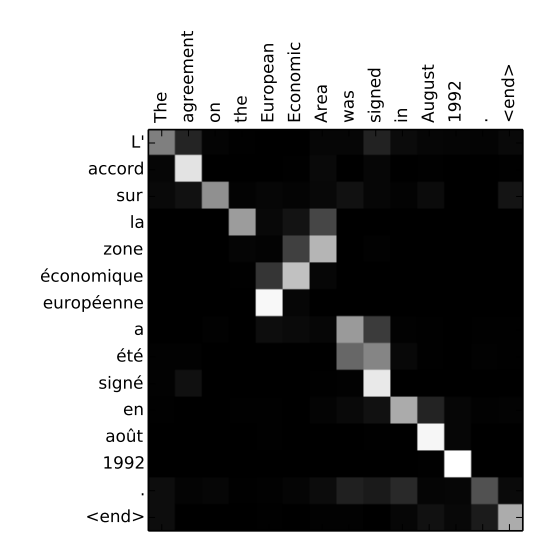
\includegraphics[width=\textwidth]{Eiropas_ekonomikas_zona}
\caption{Uzmanības mehānisma ilustrācija \cite{bahdanau2016neural}}
\label{fig:Eiropas_ekonomikas_zona}
\end{figure}

Tā ir sava veida intensitātes karte, kas norāda kur modelis “pievērš uzmanību”, kad tas izvada katru vārdu franču teikumā. Kā var redzēt, tulkojot Eiropas Ekonomiskās zonas terminu – viss termins tiek apskatīts kā saistīts kopums. Uz ko tieši modelim vērst uzmanību tiek apgūts no apmācības datiem. Veicot apmācību uz tūkstošiem franču un angļu valodas teikumu piemēriem, modelis iemācās par vārdu savstarpējo atkarību, dzimtēm, vārda formām un citiem morfoloģijas un sintakses likumiem. 

Uzmanības mehānisms ir bijis ārkārtīgi noderīgs dabīgās valodas apstrādes rīks kopš tā atklāšanas 2015. gadā, taču sākotnējā formā tas tika izmantots kopā ar rekurentiem neironu tīkliem (RNT). 

\subsubsection{Transformatora arhitektūra}

\begin{figure}[H]
	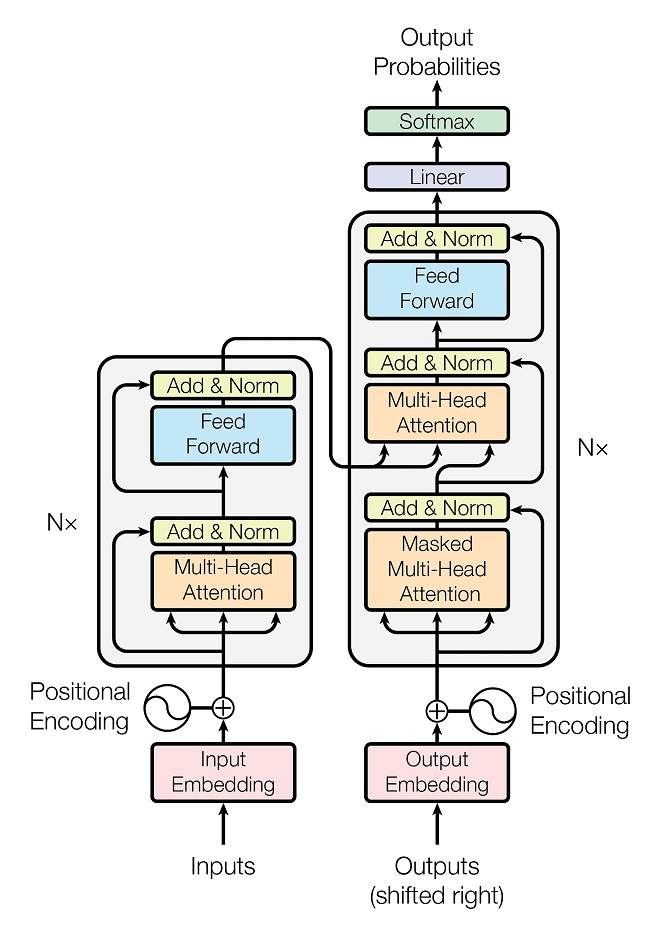
\includegraphics[scale=0.75]{attention_research}
	\caption{Transformatora arhitektūra \cite{vaswani2023attention} }
	\label{fig:vaswani2023attention_img}
\end{figure}

Transformatora arhitektūra tiek apskatīta \ref{fig:vaswani2023attention_img} attēlā. Ievade sākumā tiek padota iegulšanas slānim, kas strādā pēc principa kas jau apskatīts pie konvolūcijas neironu tīkliem - pārvēršot ievades tekstu vārdlietojuma kartējumā. Tālāk tiek veikta pozicionālā kodēšana, to savukārt var raksturot kā procesu ar kura palīdzību modelim tiek nodrošināta informācija par vārdu secību tekstā. Tas ir svarīgi tādēļ, ka transformatori apstrādā vārdus paralēli, ne secīgi, un citādāk modelim nebūtu iespējams gūt informāciju par vārdu secību/kontekstu kā tas iespējams citām arhitektūrām, piemēram, konvolūcijas neironu tīkliem vai rekurentajiem neironu tīkliem.

Katram vārdam tiek piešķirts unikāls pozīcijas  kodēšanas vektors, attēlojot vārda pozīciju tekstā. Šie pozicionālās kodēšanas vektori tiek pievienoti ievades vārdlietojuma kartējumam, papildinot katra vārda sākotnējo kartējumu, lai iekļautu informāciju par vārdus atrašanās vietu. Tas ļauj modelim arī atšķirt vārdus ar vienādu saturu, bet dažādām pozīcijām. Šo informāciju tālāk nodod pašuzmanības slānim.

Pašuzmanības slānis ir transformatora arhitektūras galvenā sastāvdaļa, nosakot kādas attiecības un atkarības starp dažādiem vārdiem ir sastopamas tekstā. Šī slāņa darbību iespējams iedalīt 4 daļās - 
\begin{itemize}
\item Vaicājumu, atslēgu un vērtību izveide
\item Uzmanības rādītāju noteikšana
\item Vairāku “uzmanības galvu” pielietojums
\item Izvades ģenerēšana
\end{itemize}

\subsubsection{Vaicājumu, atslēgu un vērtību izveide}
Lai saprastu, kā vārdi ir saistīti viens ar otru, pašuzmanības slānis katram vārdam no ievades izveido trīs vektorus

Vaicājums (Q): apzīmē vārdu, uz kuru pašlaik koncentrējamies. Katram vārdam ir atbilstošs vaicājuma vektors.

Atslēga (K): apzīmē visus vārdus, no kuriem vēlamies iegūt informāciju, lai palīdzētu noteikt katra vārda atbilstību vaicājumam.

Vērtība (V): satur informāciju par vārdiem, kurus mēs izgūsim, ja tiks atrasta atbilstība starp vaicājumu un atslēgu.

\subsubsection{Uzmanības rādītāju noteikšana}

Pašuzmanības mehānisms aprēķina uzmanības rādītājus veicot skalāro reizinājumu starp vaicājuma vektoriem (Q) un atslēgas vektoriem (K), rezultātu reizinot to ar \(\frac{1}{\sqrt{d}}\), kur d ir vaicājuma vektora garums. Papildus tam - normalizešanai tiek arī pielietota softmax funkcija. Formulu var definēt tālāk norādītā veidā.

\begin{equation}
Uzmaniba(\mathbf{Q}, \mathbf{K}, \mathbf{V}) = \text{softmax}\left(\frac{\mathbf{Q} \cdot \mathbf{K}^T}{\sqrt{d}}\right) \cdot \mathbf{V}
\end{equation}

Šie rādītāji norāda, cik daudz katram vārdam vajadzētu pievērst uzmanību citiem vārdiem. Augstāki rādītāji nozīmē lielāku uzmanību, kas liecina, ka vārds atbilst vaicājumam. Zemāki rādītāji liecina par zemāku atbilstību vai nozīmi vaicājumam. 

\subsubsection{Vairāku “uzmanības galvu” pielietojums}

Lai uzlabotu konteksta izpratni, transformators bieži izmanto vairākas vaicājumu, atslēgu un vērtību kopas, kas pazīstamas kā “uzmanības galvas”. Tas ļauj modelim vienlaikus koncentrēties uz dažādiem teksta aspektiem.

\subsubsection{Izvades ģenerēšana no pašuzmanības slāņa}
Izvade satur kontekstualizētus vārdu attēlojumus, ņemot vērā to attiecības ar citiem vārdiem. Šī izvade tagad kļūst par ievadi uz priekšu padeves (\textit{feed-forward}) slānim.

\subsubsection{Padeves slānis}
Padeves (\textit{feed forward}) slānis tiek izmantots uz pašuzmanības slāņu izvadi un tas tiek pielietots katrai pozīcijai atsevišķi. Šis slānis palīdz modelēt attālas vārdu savstarpējās atkarības. Pirmais solis padeves slānī ir lineāras transformācijas pielietošana ievadei. Tas ietver ievades reizināšanu ar apgūstamo svaru un nobīdes pievienošanu. Šī lineārā transformācija projicē ievadi citā (bieži vien augstākas dimensijas) telpā, radot pamatu sarežģītai mijiedarbībai un transformācijām. Pēc lineārās transformācijas pārveidotajai ievadei tiek piemērota nelineāra aktivizācijas funkcija, piemēram, \textit{Rectified Linear Unit} (ReLU). Aktivizācijas funkcija ievieš nelinearitāti, ļaujot modelim tvert sarežģītas saiknes datos. Pēc aktivizācijas funkcijas rezultātiem tiek piemērota cita lineāra transformācija. Šī transformācija izmanto atšķirīgus svarus un nobīdes, lai vēl vairāk pielāgotu datus.

\subsection{BERT}
BERT modelis pirmo reizi publicēts 2019. gadā un autoru vārdiem BERT ir pirmā nepārraudzītās apmācības pieeja ar dziļu divvirziena konkteksta izveidi dabīgās valodas priekšapstrādei \cite{devlin2019bert}. Viena no BERT priekšrocībām ir tā, ka visu BERT arhitektūru un jau apmācītos modeļus Google komanda ir publiskojusi caur GitHub \footnote{https://github.com/google-research/bert}, atšķirībā no citiem izplatītiem lielajiem valodas modeļiem kā GPT no OpenAI, kur modeļu izveides kods nav publiski pieejams un kuru nevaram izmantot darbā apskatītās problēmas risināšanai.

Ar BERT arhitektūru tiek apmācīts “valodas izpratnes” modelis, izmantojot lielapjoma teksta korpusus, piemēram, visus Wikipedia rakstus konkrētajā valodā. Pēc tam jāveic modeļa pielāgošana konkrētu dabīgās valodas apstrādes uzdevumu risināšanai kā tekstu klasifikācija. Nepārraudzītā apmācība ļauj veidot BERT modeli uz plašiem teksta korpusiem no jebkura interneta resursa.

Svarīga loma iekš BERT ir arī kā valodas dati tiek vektorizēti. Valodas attēlojumi vektora formā var iekļaut sevī kontekstu un var neiekļaut to. Citas iepriekš populārākās vektorizācijas pieejas kā word2vec ģenerē vārdlietojuma kartējumu bez konteksta katram vārdam apmācības vārdnīcā, respektīvi, daudznozīmīgi vārdi (piemēram, "komanda" - ko varam uztvert kā pavēli vai cilvēku kopu sportā) pazaudē savu atšķirīgo nozīmi un patieso kontekstu. Kontekstu veidojoši modeļi savukārt ģenerē attēlojumu katram vārdam atkarībā no konteksta konkrētajā teikumā. BERT gadījumā, atšķirībā no citiem iepriekšējiem modeļiem, šis konteksts tiek veidots divos virzienos – apskatot vārdus gan pirms, gan pēc konkrētā vārda. Šādai priekšapstrādei BERT izmanto sekojošu pieeju -  tiek maskēti 15\% ievades vārdu, tālāk šādu ievades kopu apstrādā caur dziļu divvirzienu transformatora kodētāju, pēc tam paredz tikai maskētos vārdus. Piemēram:

Ievade: vīrietis devās uz [MASK1]. Viņš nopirka [MASK2] piena.

Etiķetes: [MASK1] = veikalu; [MASK2] = litru

Papildus, lai apmācītu arī attiecības starp teikumiem, tiek veikta apmācība uz vienkāršu uzdevumu, kurš pielietojams jebkuram valodas korpusam. Šis uzdevums ir - ja doti divi teikumi A un B, vai B ir nākamais teikums, kas seko aiz A, vai arī vienkārši nejaušs teikums no valodas korpusa? Piemērs varētu izskatīties šādi.

Teikums A: Vīrietis devās uz veikalu.

Teikums B: Viņš nopirka litru piena.

Pazīme: IsNextSentence

Teikums A: Vīrietis devās uz veikalu.

Teikums B: Pingvīni nelido.

Pazīme: NotNextSentence

\section{Modeļu novērtēšana un validācija}
Pēc apmācīta modeļa iegūšanas ir svarīgi novērtēt izveidotā modeļa veiktspēju un to, cik labi tas spēs veikt tekstu klasifikāciju ar jauniem datiem. 
Viena no izplatītākajām novērtēšanas metodēm ir metode ar noturēšanu (\textit{holdout method}), kur paraugu kopa tiek sadalīta divās daļās – apmācības kopa un testa kopa. Klasifikators tad tiek apmācīts ar apmācību kopu un validēts ar testa kopu. Šīs metodes mīnuss ir tas, ka apmācībai pieejama mazāka datu kopa. Cita negatīvā īpašība šai metodei ir arī tā, ka rezultāti ir atkarīgi no nevienlīdzīgā datu sadalījuma starp šīm abām kopām.

Cita metode ir nejauša paraugu atlase (\textit{Random Subsampling}). Šī metode atkārto metodi ar noturēšanu vairākas reizes, lai labāk noteiktu modeļa veiktspēju, tomēr arī šai metodei piemīt pirmās metodes negatīvās īpašības.
Modeļa novērtēšana ar apmācību datiem nav ieteicama, jo tādējādi notiks pārmērīga pielāgošana (\textit{overfitting}) un mašīnmācīšanās modelis iegaumēs apmācības datus, bet nespēs pareizi klasificēt jaunus datus.

Visbeidzot var izmantot arī šķērsvalidāciju (\textit{cross-validation}). Šī metode sadala paraugu kopu k vienādās daļās un izmanto katru no šīm daļām tieši vienu reizi priekš testēšanas.  Citas, k-1, reizes katra daļa tiek izmantota apmācībai.

\subsubsection{Klasifikācijas mēri}
\renewcommand{\theequation}{2.\arabic{equation}}
Klasifikācijas problēma ir bieži apskatīts mašīnmācīšanās temats un visizplatītākie mēri, ar kuriem novērtēt modeļa precizitāti ir aprakstīti zemāk.

\subsubsection{Pārpratumu matrica}
Pārpratumu matrica ļauj pārredzami attēlot modeļa precizitāti modelim ar divām un vairāk klasēm. Matrica sastāv no divām asīm, kur uz x ass tiek attēlotas visas klases un uz y ass tiek attēloti klases minējumi. Katra matricas šūna satur minējumu skaitu attiecīgajai klases un minētās klases kombinācijai.

Bināras klasifikācijas gadījumā pārpratumu matrica varētu būt attēlojama ar šādu tabulu:
\begin{table}[H]
\centering
\caption{\label{tab:novertejums}}
\textbf{Pārpratuma matrica\\}
\begin{tabular}{|l|l|l|}
\hline
  & +  & -  \\ \hline
+ & PA & KA \\ \hline
- & KN & PN \\ \hline
\end{tabular}
\end{table}

Kur tabulas  \ref{tab:novertejums} vērtības raksturojamas šādi:
\begin{itemize}
\item PA - pareiza atbilsme (tabulā - gadījumi, kad '+' tiek pareizi klasificēts)
\item PN - pareiza neatbilsme (tabulā - gadījumi, kad '-' tiek pareizi klasificēts)
\item KA - kļūdaina atbilsme (tabulā - gadījumi, kad '-' tiek nepareizi klasificēts kā '+')
\item KN - kļūdaina neatbilsme (tabulā - gadījumi, kad '+' tiek nepareizi klasificēts kā '-')

\end{itemize}
\subsubsection{Akurātums}
Akurātums ir mērs, kurš norāda cik no minējumiem ir bijuši pareizi. Tas ir pareizo minējumu dalījums ar visu minējumu skaitu.
\begin{equation}
Akur\bar{a}tums = \frac{PA + PN}{PA + PN + KA + KN}
\end{equation}
\subsubsection{Precizitāte}
Precizitāte ir mērs, kas parāda pareizo pozitīvo vērtību proporciju starp modeļa kopējiem pozitīvajiem minējumiem. Tas atbild uz jautājumu "Cik no visām veiktajām pozitīvajām prognozēm bija patiesas?". Tas ir svarīgs mērs gadījumos, kad svarīgi ir novērst tieši kļūdaini pozitīvus minējumus.
\begin{equation}
Precizit\bar{a}te = \frac{PA}{PA + KA}
\end{equation}
\subsubsection{Pārklājums}
Pārklājums norāda uz to, cik labi modelis spēj atrast visas pozitīvās vērtības. Šis mērs atbild uz jautājumu "Cik no visiem datu punktiem, kas būtu jāparedz kā patiesi, tika pareizi prognozēti kā patiesi?". Tas ir svarīgs mērs gadījumos, kad svarīgi ir novērst tieši kļūdaini negatīvus minējumus.
\begin{equation}
P\bar{a}rkl\bar{a}jums = \frac{PA}{PA + KN}
\end{equation}
\subsubsection{F1 mērs}
F1 mērs ir precizitātes un pārklājuma mēru harmoniskais vidējais.
\begin{equation}
F1 = \frac{(2 * precizit\bar{a}te * p\bar{a}rkl\bar{a}jums)}{(precizit\bar{a}te + p\bar{a}rkl\bar{a}jums)}
\end{equation}
Atšķirībā no aritmētiskas vidējās vērtības, harmoniska vidējā vērtība tiecas uz mazāko vērtību no diviem mēriem, no tā izriet, ka F1 mērs būs zems ja precizitāte vai pārklājums ir zems. Īpaši noderīgs šis mērs ir gadījumos, kad vēlamies noteikt modeļa veiktspēju datu kopā ar nevienmērīgu klašu sadalījumu.

\section{Biežākās problēmas tekstu klasifikācijā}
\subsubsection{Morfoloģiskā un sintaktiskā sarežģītība}
Liela nozīme ir konkrētai valodai, kurai veicam apstrādi. Darbā apskatam latviešu valodu un tā gan morfoloģiski, gan sintaktiski ir  sarežģītāka par izplatītākām valodām kā angļu valodu \cite{morphologicalComplexity}, kurai dabīgās valodas apstrāde ir pētīta visplašāk. Morfoloģiskā sarežģītība Eiropā izplatītajām valodām apskatīta attēlā \ref{fig:morfologiska_sarezgitiba}.
 \begin{figure}[H]
	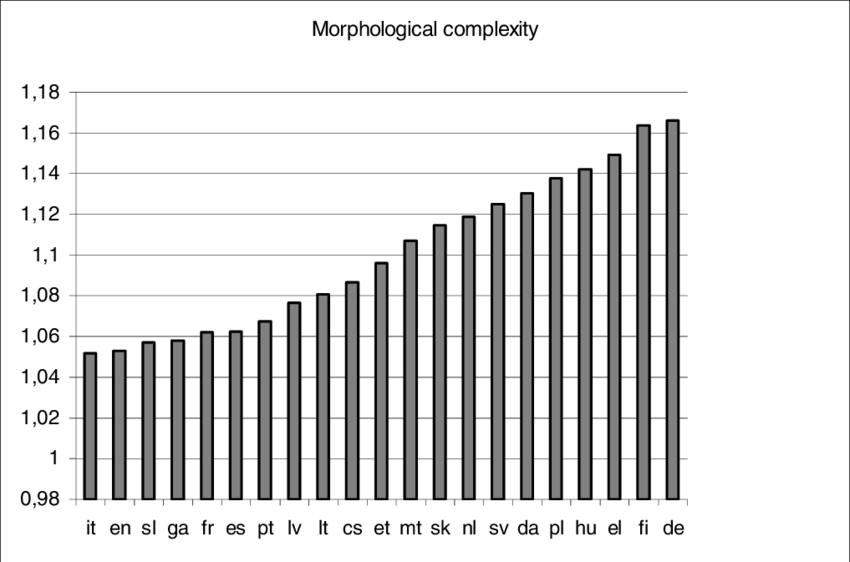
\includegraphics[width=\textwidth]{Morphological-complexity}
	\caption{Morfoloģiskā sarežģītība Eiropas valodām\cite{morphologicalComplexity}}
	\label{fig:morfologiska_sarezgitiba}
\end{figure}
 
Papildus tam - dabiskā valoda var būt neskaidra, ar vārdiem un frāzēm, kuriem ir vairākas nozīmes atkarībā no konteksta. Šīs neskaidrības precīza risināšana ir izaicinājums teksta klasifikācijas modeļiem.

\subsubsection{Tekstu nevienmērība}
Teksta dati ir dažādi un atšķiras pēc garuma, struktūras un kvalitātes. Tie var ietvert konkrētu autoru tipiskās kļūdas, slengu, saīsinājumus un plašu rakstīšanas stilu klāstu, kas padara tos grūti standartizējamus. Arī kopumā bieži apmācībai pieejamie dati nav vienmērīgi - dažādas tekstu klases var būt vai nu plašāk vai retāk izplatītas dotā datu kopā.

\subsubsection{Pārmērīga pielāgošana}
Pārmērīga pielāgošana nozīmē to, ka klasifikators ir pārāk labi modelējis apmācības datus
un nedarbojas labi uz iepriekš neredzētiem datiem. Kļūdas, ko klasifikators pieļauj uz apmācības datiem sauc par apmācības kļūdām, savukārt kļūdas, kuras tiek pieļautas uz iepriekš neredzētiem datiem, sauc par vispārināšanas kļūdām. Labam modelim ir gan zems apmācības kļūdu skaits, gan zems vispārināšanas kļūdu skaits. Nepietiekama pielāgošana notiek ja modelim ir gan augsts apmācības kļūdu skaits, gan arī augsts vispārinājuma kļūdu skaits. No otras puses - pārmērīga pielāgošana notiek kad modelim ir zems apmācības kļūdu skaits, bet augsts vispārināšanas kļūdu skaits \cite{tan2005introduction}. Zemāk apskatāmajā attēlā \ref{fig:pielagosana} attēloti piemēri divdimensiju klasifikācijas scenārijā.

\begin{figure}[H]
	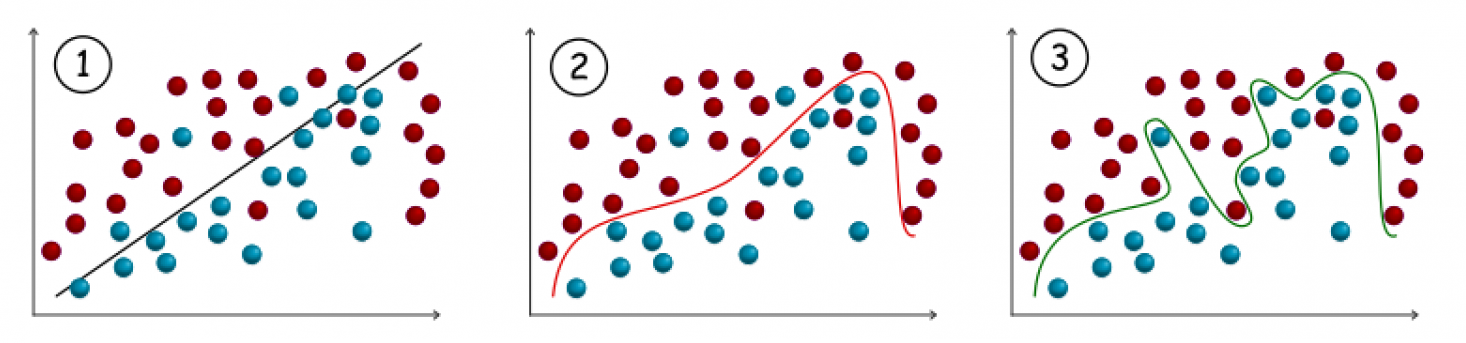
\includegraphics[width=\textwidth]{pielagosana}
	\caption{Pielāgošanas scenāriji (1 - nepietiekama, 2 - optimāla, 3 - pārmērīga)}
	\label{fig:pielagosana}
\end{figure}
 
Visbiežāk šāda veida kļūdas rodas no apmācību datiem, kuros ir pārāk daudz ar konkrēto klasifikāciju nesaistīti dati (lieks fona “troksnis”) vai arī izvēlētais apmācību datu apjoms ir pārāk mazs.


\chapter{Rāpuļa un klasifikācijas modeļu izveide}
\section{Datu izgūšana no ziņu portāliem ar rāpuli}
Lai veiktu izpēti, sakumā ir nepieciešams ievākt treniņdatus / valodas korpusu, kas raksturo problēmvidi – ziņu portālu rakstus. Praktiskai rāpuļa implementācijai tika izvēlēts \textit{Python} ietvars \textit{Scrapy}, ar kura palīdzību iespējams izveidot tīmekļa rāpuļus, kas pārmeklē mājaslapas un izvelk no tām datus strukturētā formā. Šis ietvars izvēlēts, jo tas ir viens no populārākajiem rīkiem šajā kategorijā un tas labi spēj apstrādāt un formatēt lielu datu apjomu. Tā kā tīmekļa rāpuļi ir jāpielāgo konkrētai mājaslapas struktūrai, lai iegūtu vēlamos datus, tika izvēlēts konkrēts portāls - delfi.lv, dēļ tā daudzveidīgā kategoriju klāsta un rakstu daudzuma. Lai palielinātu iegūstamo rakstu daudzveidību tika apsvērts pielietot rāpuli arī uz citiem ziņu portāliem, tomēr tiem visiem ir liels pārklājums savā starpā, pārpublicējot rakstus no ziņu aģentūrām kā LETA. Šāda pieeja sekojoši varētu novest pie dublikātiem datu kopā, radot iespēju vienādiem rakstiem parādīties gan apmācības, gan validācijas kopās vienlaicīgi. Darba ietvaros izveidots rāpulis, kas ievāc datus no delfi.lv portāla un saglabā tos JSON formā ar 4 pamatlaukiem – virsraksts, kategorija, saturs, hipersaite. Lai sašaurinātu problēmvidi un ierobežotu nepieciešamos resursus tika izvēlētas 10 apskatāmās kategorijas – mūzika, atpūta, kriminālziņas, finanses, tehnoloģijas, kino, literatūra, politika, sports, auto. Darbības princips rāpulim ir kā norādīts tālāk.
\begin{itemize}
\item Rāpulim sākotnēji apskatāmās saites tiek norādītas kā 10 izvēlēto kategoriju lapas (piemēram, politikas ziņām - https://www.delfi.lv/193/politics?page=1).
\item No lapām tiek iegūtas hipersaites uz individuāliem rakstiem, ierobežojot tālāk apskatāmās saites tā, lai tās aizvien piederētu apskatāmajām kategorijām un nesaturētu nevēlamas saites (kā komentāru lapas rakstiem).
\item Tiek apstrādāta katra raksta lapu, piefiksējot hipersaiti un dažādas komponentes - virsrakstu, kategoriju, saturu, atlasot tos pēc HTML elementu atbilstības konkrētas komponentes kritērijiem.
\item Katrs raksts tiek saglabāts JSON formātā un ierakstīts failā, atkārtojot procedūru līdz vairs netiek atrasti unikāli raksti ko rāpulim apmeklēt.
\end{itemize}

\textit{Scrapy} ietvars kopumā dod iespēju diezgan efektīvi realizēt šādu rāpuli – sākot no apskatāmo rakstu ierobežošanas līdz elementu atlasei un apstrādei. Salīdzinoši grūtāk ir tieši formalizēt kādus selektorus izvēlēties elementu atlasei, jo lapu formatējums starp dažādām kategorijām mēdz būt atšķirīgs un pat vienas kategorijas ietvaros tika novērots ka senākiem rakstiem formatējums var atšķirties no jaunāko rakstu formatējuma. Papildus tam arī ne visi raksti ir derīgi datu ieguvei, piemēram sastopami raksti kas satur tikai foto un video galerijas ar minimāliem aprakstiem, sastopami arī maksas raksti ar tikai vienu publiski pieejamu rindkopu.

Izgūta raksta piemēru JSON formātā iespējams apskatīt \ref{appendix:raksta_piemers} pielikumā. Rezultātā tika ievākti 13762 raksti ar sadalījumu pa kategorijām kāds redzams \ref{tab:rakstu_kategorijas} tabulā.
\begin{table}[H]
\centering
\caption{\label{tab:rakstu_kategorijas}}
\textbf{Ievākto rakstu sadalījums pa kategorijām\\}
\begin{tblr}{
  hlines,
  vlines,
}
Kategorija    & Raksti  \\
Mūzika & 1722  \\
Atpūta & 1523  \\
Kriminālziņas & 1517  \\
Finanses & 1363  \\
Tehnoloģijas & 1333  \\
Kino & 1282  \\
Literatūra & 1277  \\
Politika & 1263  \\
Sports & 1250  \\
Auto & 1232
\end{tblr}
\end{table}

Ar rāpuli izgūtie teksti papildus tika manuāli pārbaudīti un attīrīti no nevēlamiem datiem – iegulti koda fragmenti audio /video atskaņotājiem, hipersaites. Ievācot rakstus novērots, ka bez rakstu satura atšķiras arī vidējie rakstu garumi katrā kategorijā. Piemēram atpūtas ziņām raksturīgi gari raksti ar vidēji vairāk nekā 662 vārdiem, savukārt auto, sporta un kriminālziņām – krietni īsāki raksti (īpaši auto ziņām ar vidējo rakstu garumu ap 227 vārdiem). Šāda atšķirība garumos varētu atstāt ietekmi uz konkrētu kategoriju klasifikāciju akurātumu. Rakstu iedalījumu garumos sīkāk iespējams apskatīt \ref{appendix:kategorijas_wc} pielikumā.

Rāpuļa kods pieejams \ref{appendix:code_repo} pielikuma 1. repozitorijā.

\section{Klasisko mašīnmācīšanās algortimu implementācija}

\subsubsection{Izmantotie rīki}
Viena no \textit{Python} valodas populārākajām mašīnmācīšanās bibliotēkām, kas palīdz risināt problēmas kā klasteru veidošana, regresija, klasifikācija, dimensiju skaita samazināšana, ir \textit{sckit-learn}. Autors ir izvēlējies lietot šo bibliotēku lai atvieglotu plaši lietotu klasifikācijas algoritmu implementāciju (Naivā Bejesa metode, loģistiskā regresija, lēmumu koki,  atbalsta vektoru mašīnas). 

Svarīga loma valodas apstrādē arī ir ievades tokenizācijai, tās veikšanai iespējams izmantot Python bibliotēkas kā \textit{NLTK} un \textit{spaCy}. Tieši šīs divas bibliotēkas ir populārākās un spēj tikt galā ar biežām tokenizācijas problēmām kā saīsinājumu, pieturzīmju un simbolu atdalīšana. Darba ietvaros tokenizācijas nolūkiem tika izvēlēts pielietot \textit{spaCy}.

\subsection{Priekšapstrāde un vektorizācija}
\subsubsection{Tokenizācija un tekstu attīrīšana}
Teksta apstrāde tiek sākta ar teksta tokenizāciju, izmantojot \textit{spaCy} bibliotēkā iebūvētās metodes. Kad teksts ir sadalīts vārdos – apstrāde tiek turpināta ar visu vārdu pārvēršanu formā ar visiem mazajiem burtiem, tiek izņemtas pieturzīmes un stopvārdi.

Konkrētāk apskatot stopvārdu atmešanu - dažādās \textit{Python} bibliotēkās ir iekļauti saraksti ar stopvārdiem izplatītām valodām, tomēr latviešu valodai šāds sarakts jādefinē neatkarīgi. Tika veikta izpēte par to vai šāds saraksts jau ir publiski pieejams un kā viens no populārākajiem atrasts ''stopwords-lv'' repozitorijs \footnote{https://github.com/stopwords-iso/stopwords-lv}) . Lai gan tas ir izmantojams kā labs pamats un uzskaita palīgvārdus (saikļus, prievārdus, partikulas), trūkst citas svarīgas morfoloģiskās grupas kā vietniekvārdi (attieksmes vietniekvārdi – kurš, kura u.c., norādāmie vietniekvārdi – šis, šī, tas, tā, viņš u.c, kā arī locījumi šiem vārdiem), jo arī šo vārdu esamība neraksturo teksta fragmenta jēgu vai piederību kādai kategorijai. Darba ietvaros izveidots uzlabots stopvārdu saraksts latviešu valodai, kas labāk spētu veikt vārdu filtrēšanas soli teksta priekšasptrādē, un pielietots uz apmācības datiem. 

Lemmatizācija netiek pielietota, dazādiem autoriem norādot tās mazo nozīmi tekstu klasifikācijas modeļu uzlabošanā \cite{santos2023effect}. Citos pētījumos, piemēram par angļu un čehu valodas datu kopu priekšapstrādi \cite{normalizationTextClassification}, secināts, ka kopumā stopvārdu izņemana gandrīz vienmēr uzlabo iegūtos rezultātus, tomēr lemmatizācija gandrīz vienmēr atstāj negatīvu ietekmi uz gala modeli.

\subsubsection{Vektorizācija}
Pirms algoritmu pielietošanas nepieciešams datus vektorizēt. Darba ietvaros uz katru no algoritmiem tika pārbaudītas dažādas vektorizācijas pieejas – vārdu maiss, bigrammu maiss, TF-IDF un vārdlietojuma kartējumi ar \textit{FastText}, pielietojot katru no tām uz rāpuļa izgūtās datu kopas. Tika arī veikti eksperimenti ar \textit{word2vec} vārdlietojuma kartējuma pieeju, tomēr \textit{FastText} pielietošana sniedza labākus sākotnējos rezultātus, arī citi pētījumi par vārdlietojuma kartējuma pieejām latviešu valodas tekstiem \cite{LaucisJekabsonWordEmbedding} norāda \textit{FastText} kā pieeju ar labāko veiktspēju, salīdzinot ar \textit{word2vec}, \textit{ngram2vec}, SSG (\textit{Structured Skip-Gram}).

FastText gadījumā tiek lietots jau apmācīts vārdu vektors, apmācīts uz \textit{Common Crawl} \footnote{https://commoncrawl.org/} rāpuļa un \textit{Wikipedia} rakstu kopām latviešu valodā. Vārdu vcktors ir publicēts FastText oficiālajā mājaslapā \footnote{https://fasttext.cc/docs/en/crawl-vectors.html} un tiek pielietots kodā caur \textit{Gensim} bibliotēku.

\subsection{Algoritmu implementācijas}

\subsubsection{Datu līdzsvarošana un sadale}
Svarīgs priekšnosacījums labai klasifikācijas modeļa apmācībai ir izvairīšanās no nevienmērīga klašu sadalījuma datu kopā. Ar rāpuli tika mēģināts izgūt samērā līdzīgu rakstu skaitu pa kategorijām, tomēr atšķirības eksistē, piemēram, klasei “Mūzika” rezultātā tika izgūti 1722 raksti, bet auto ziņām – 1232 raksti. Pirms apmācības visām kategorijām saglabājam 1200 rakstus, pārējos atmetot. Rezultātā iegūstam 12 000 rakstus, kurus tālāk sadalām – 80\% apmācībai (9600 raksti), 20\% validācijai (2400 raksti).

\subsubsection{Atbalsta vektora mašīnas}
Atbalsta vektora mašīnas apmācības algoritms ir implementēts ar \textit{scikit-learn} komponenti \textit{LinearSVC} (sklearn.svm.LinearSVC) ar dažādām vektorizācijas metodēm. Novērtēto akurātuma mēru ar dažādām vekorizācijas pieejām varam apskatīt \ref{tab:accuracy_svm} tabulā.
\begin{table}[H]
\centering
\caption{\label{tab:accuracy_svm}}
\textbf{Akurātuma mēri pielietojot AVM\\}
\begin{tabular}{|l||l|l|l|l|}
\hline
& Vārdu maiss & Bigrammu maiss & TF-IDF & FastText \\ \hline
Akurātums & 0.9696 & 0.9679 & \textbf{0.9738} & 0.9596 \\ \hline
F1 & 0.9695 & 0.9678 & \textbf{0.9737} & 0.9594 \\ \hline
\end{tabular}
\end{table}

\subsubsection{Naivā Bajesa metode}
Naivā Bajesa apmācības algoritms ir implementēts ar \textit{scikit-learn} komponenti \textit{MultinomialNB} (sklearn.naive\_bayes.MultinomialNB) ar dažādām vektorizācijas metodēm. Novērtēto akurātuma mēru ar dažādām vekorizācijas pieejām varam apskatīt \ref{tab:accuracy_nb} tabulā.
\begin{table}[H]
\centering
\caption{\label{tab:accuracy_nb}}
\textbf{Akurātuma mēri pielietojot Naivā Bajesa metodi\\}
\begin{tabular}{|l||l|l|l|l|}
\hline
& Vārdu maiss & Bigrammu maiss & TF-IDF & FastText \\ \hline
Akurātums & \textbf{0.9629} & 0.9558 & 0.9617 & 0.8758 \\ \hline
F1 & \textbf{0.9628} & 0.9559 & 0.9616 & 0.8757 \\ \hline
\end{tabular}
\end{table}

\subsubsection{Loģistiskā regresija}
Loģistiskās regresijas apmācības algoritms ir implementēts ar \textit{scikit-learn} komponenti \textit{LogisticRegression} (sklearn.linear\_model.LogisticRegression) ar dažādām vektorizācijas metodēm. Novērtēto akurātuma mēru ar dažādām vekorizācijas pieejām varam apskatīt \ref{tab:accuracy_lr} tabulā.

\begin{table}[H]
\centering
\caption{\label{tab:accuracy_lr}}
\textbf{Akurātuma mēri pielietojot loģistisko regresiju\\}
\begin{tabular}{|l||l|l|l|l|}
\hline
& Vārdu maiss & Bigrammu maiss & TF-IDF & FastText \\ \hline
Akurātums &  \textbf{0.9663} & 0.9633 &  \textbf{0.9663} & 0.9575 \\ \hline
F1 &  \textbf{0.9662} & 0.9633 &  \textbf{0.9662} & 0.9574 \\ \hline
\end{tabular}
\end{table}

\subsubsection{Lēmumu koki}
Lēmumu koku pmācības algoritms ir implementēts ar \textit{scikit-learn} komponenti \textit{DecisionTreeClassifier} (sklearn.tree.DecisionTreeClassifier) ar dažādām vektorizācijas metodēm. Novērtēto akurātuma mēru ar dažādām vekorizācijas pieejām varam apskatīt \ref{tab:accuracy_dt}tabulā.

\begin{table}[H]
\centering
\caption{\label{tab:accuracy_dt}}
\textbf{Akurātuma mēri pielietojot lēmumu kokus\\}
\begin{tabular}{|l||l|l|l|l|}
\hline
& Vārdu maiss & Bigrammu maiss & TF-IDF & FastText \\ \hline
Akurātums & 0.8129 & \textbf{0.8250} & 0.8 & 0.7529 \\ \hline
F1 & 0.8129 & \textbf{0.8249} & 0.8004 & 0.7517 \\ \hline
\end{tabular}
\end{table}

\subsubsection{Priekšapstrādes nozīme un rezultātu salīdzinājums}

Lai veiksmīgi varētu novērtēt priekšapstrādes lomu modeļu veiktspējā, iepriekš apskatītie algoritmi un vektorizācijas pieejas tiek pārbaudīti arī bez tekstu papildus priekšapstrādes. Īpaši nozīmīgi tas ir modeļiem ar FastText vektorizāciju, jo šajā gadījumā priekšapmācītie vārdu vektori ir apmācīti bez priekšapstrādes \cite{grave2018learning}. Rezultāti apkopoti tabulā \ref{tab:accuracy_all}, izceļot labākos rezultātus starp pieejām ar priekšapstrādi un bez tās.

\begin{table}[H]
\centering
\caption{\label{tab:accuracy_all}}
\textbf{Akurātuma mēri dažādiem modeļiem ar un bez priekšapstrādes\\}
\begin{tabular}{|l|l|l|}
\hline
                                         & \makecell{Ar \\ priekšapstrādi} & \makecell{Bez \\ priekšapstrādes}  \\ \hline
Atbalsta vektora mašīna (TF-IDF)         & 0.9738   & \textbf{\textcolor{teal}{0.9746}}  \\ \hline
Atbalsta vektora mašīna (Bigrammu maiss) & \textbf{0.9679}   & 0.9642\\ \hline
Atbalsta vektora mašīna (Vārdu maiss)    & \textbf{0.9696}   & 0.9667  \\ \hline
Atbalsta vektora mašīna (FastText)       & \textbf{0.9596}            & 0.9592 \\ \hline
Naivā Bajesa metode (TF-IDF)             & \textbf{0.9617}   & 0.9537 \\ \hline
Naivā Bajesa metode (Bigrammu maiss)     & \textbf{0.9558}   & 0.94  \\ \hline
Naivā Bajesa metode (Vārdu maiss)        & \textbf{0.9629}   & 0.9567 \\ \hline
Naivā Bajesa metode (FastText)           & \textbf{0.8758}     & 0.8396 \\ \hline
Loģistiskā regresija (TF-IDF)            & \textbf{0.9663}            & 0.9625 \\ \hline
Loģistiskā regresija (Bigrammu maiss)    & \textbf{0.9633}   & 0.9567 \\ \hline
Loģistiskā regresija (Vārdu maiss)       & \textbf{0.9663}   & 0.9550 \\ \hline
Loģistiskā regresija (FastText)          & \textbf{0.9575}   & 0.9558 \\ \hline
Lēmumu koki (TF-IDF)                     & \textbf{0.8}   & 0.7850 \\ \hline
Lēmumu koki (Bigrammu maiss)             & \textbf{0.8250}   & 0.7979  \\ \hline
Lēmumu koki (Vārdu maiss)                & \textbf{0.8129}            & 0.7992 \\ \hline
Lēmumu koki (FastText)                   & \textbf{0.7529}   & 0.7308 \\ \hline
\end{tabular}
\end{table}

Pēc tabulas datiem varam novērot, ka priekšapstrāde gandrīz vienmēr uzlabo gala rezultātu, lai gan sastopami arī izņēmums tieši modelī ar labāko rezultātu. Kopumā gan priekšapstrādes ietekme nav vērtējama kā pārāk liela – labākajam modelim sniedzot akurātuma uzlabojumu kā 0,0008. 

Vislabākais sasniegtais akurātums iegūts ar atbalsta vektora mašīnām un TF-IDF vektorizāciju - \textbf{0.9738}, šai pieejai varam vizualizēt kategorizāciju ar pārpratuma matricu. Kā redzams \ref{fig:AVM_TFIDF} attēlā – desmit  kategoriju klasifikācija tiek veikta ļoti precīzi un biežākā kļūda ir nepareizi klasificētas finanšu ziņas, klasificējot tās kā tehnoloģiju ziņas.

\begin{figure}[H]
	\centering
	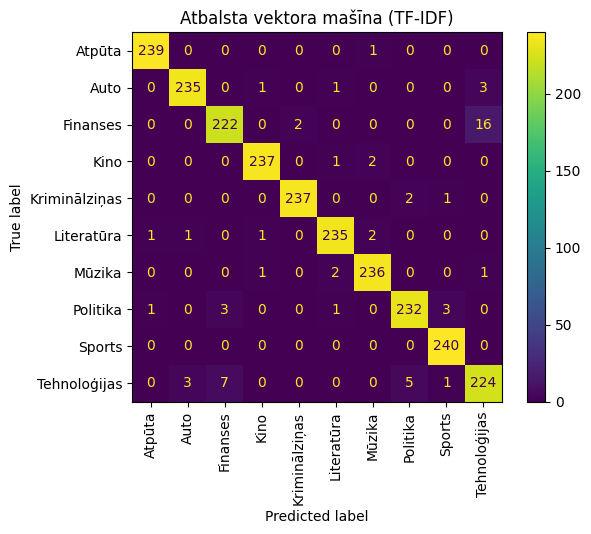
\includegraphics[width=0.75\textwidth]{AVM_TFIDF}
	\caption{Atbalsta vektora mašīnas pārpratuma matrica}
	\label{fig:AVM_TFIDF}
\end{figure}

\pagebreak
\section{Neironu tīklu implementācija}

Darba ietvaros tika izvērtētas un implementētas dažādas neironu tīklu arhitektūras. Tā kā tika nolemts pārbaudīt plašu spektru ar dažādiem apmācības algoritmiem – tika izvēlēts Python ietvars \textit{Keras}, balstīts uz \textit{Tensorflow} bāzes, kas palīdz ātri un sintaktiski vienkārši prototipēt dažādus modeļus. Neironu tīklu apmācība, vismaz sākotnēji, tika veikta uz autora datora, izmantojot viduvējas veiktspējas procesoru (AMD Ryzen 5700X) un 16GB RAM. Apmācība vienkāršākiem tīkliem šādi veicama diezgan efektīvi, tomēr sarežģītākas arhitektūras ar BiLSTM slāņiem vai BERT modeļa pielāgošana kļūst gan laikietilpīgāka (12+ stundu apmācība), gan ierobežota operatīvās atmiņas resursu dēļ. Šo iemeslu dēļ darba gaitā modeļu apmācība turpināta ar Google TPU v2, kas izstrādāts tieši neironu tīklu apmācībai un nodrošina krietni ātrakus apmācību laikus.

\subsection{Konvolūcijas neironu tīkli}
Konvolūcijas tīklu implementācijai tiek veidots Keras modelis ar secīgiem slāņiem – iegulšanas, viendimensiju konvolūcijas ar ReLU aktivizācijas funkciju, apvienošanas (globālā maksimuma), atmešanas, pilnīgi savienotais slānis gala klasifikācijas veikšanai. Ilustrēti ar papildus informāciju par izvēlētajām slāņu dimensijām varam apskatīt modeli \ref{fig:SingleLayerCNN} attēlā.

\begin{figure}[H]
	\centering
	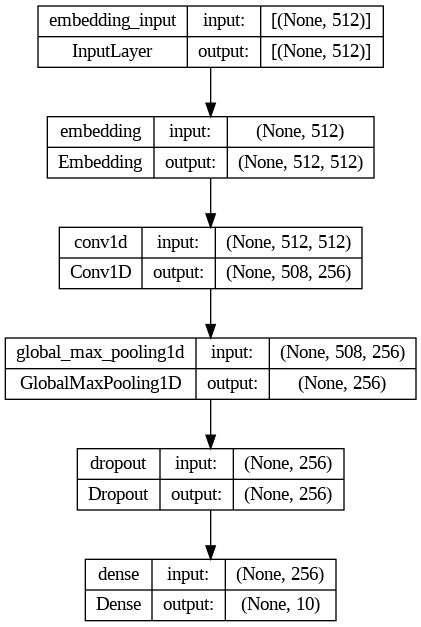
\includegraphics[width=0.4\textwidth]{SingleLayerCNN}
	\caption{Konvolūcijas neironu tīkla uzbūve}
	\label{fig:SingleLayerCNN}
\end{figure}

\pagebreak
Apmācība tiek veikta ar partijas izmēru kā 32, turpinot apmācību 10 epohos, saglabājot modeli posmos ar mazāko validācijas zuduma (\textit{validation loss}) vērtību, mēģinot izvairīties no pārmērīgas pielāgošanas. Uz tekstiem pirms apmācības tiek veikta priekšapstrāde - simbolu un stopvārdu atmešana. Akurātuma un zuduma evolūciju pa epohiem iespējams apskatīt \ref{fig:Accuracy_Loss_CNN_10epoch} attēlā.

\begin{table}[H]
\centering
\caption{\label{tab:score_cnn}}
\textbf{Veiktspējas mēri pielietojot konvolūcijas neironu tīklu\\}
\begin{tabular}{|l|l|}
\hline
Akurātums & F1 \\ \hline
0.9617 & 0.9616  \\ \hline
\end{tabular}
\end{table}

Pielietojot attēlā \ref{fig:SingleLayerCNN} ilustrēto konvolūcijas neironu tīkla uzbūvi tiek iegūti rezultāti kā \ref{tab:score_cnn} tabulā. Pārpratuma matricu iespējams apskatīt \ref{fig:CNN} attēlā, kur varam novērot līdzīgu kļūdu izplatību pa klasēm kā iepriekš apskatītos modeļos, arī ar šo pieeju visgrūtāk modelim ir atķirt tieši tehnoloģiju un finanšu ziņas.

\begin{figure}[H]
	\centering
	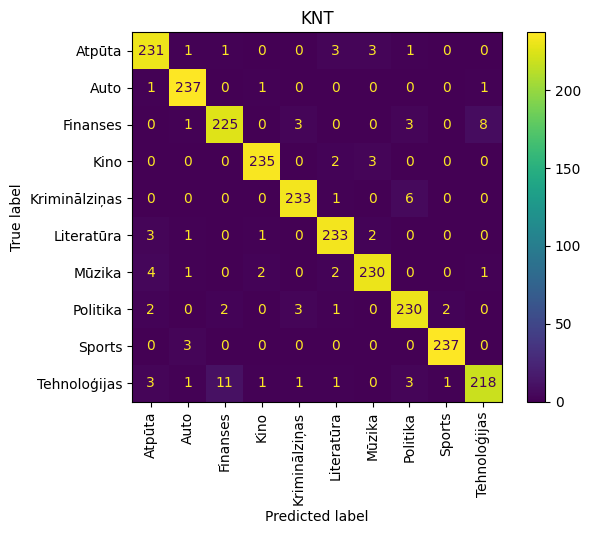
\includegraphics[width=0.75\textwidth]{CNN}
	\caption{Konvolūcijas neironu tīkli - pārpratuma matrica}
	\label{fig:CNN}
\end{figure}

\begin{figure}[H]
	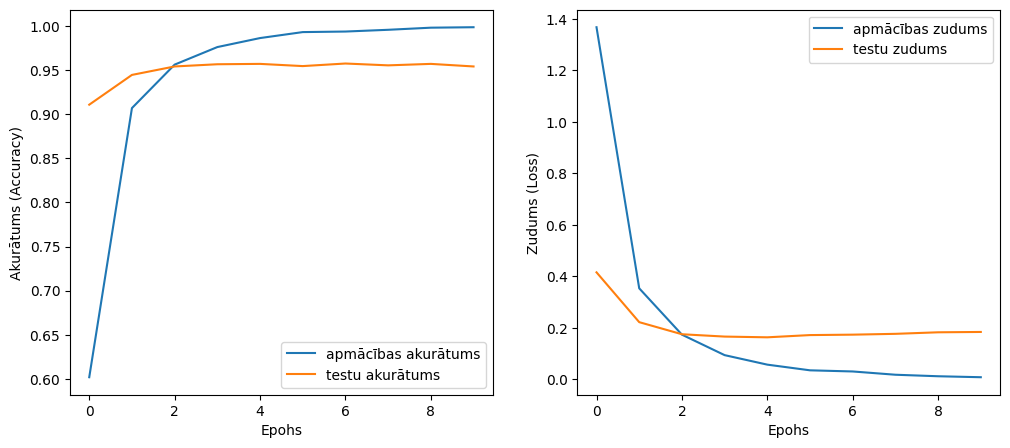
\includegraphics[width=\textwidth]{Accuracy_Loss_CNN_10epoch}
	\caption{Konvolūcijas neironu tīkli - novērtējums pa apmācības posmiem}
	\label{fig:Accuracy_Loss_CNN_10epoch}
\end{figure}

Mēģinot uzlabot modeļa veiktspēju tiek pielietota plaši citēta konvolūcijas neironu tīklu arhitektūra tekstu apstrādei no Kim Yoon \cite{kimYoonCNN}. Šīs arhitektūras galvenā ideja ir ieviest vairākus paralēlu konvolūcijas un apvienošanas slāņus ar dažādiem filtra izmēriem, vēlāk to rezultātus apkopojot. Galvenais iemesls – palīdzēt neironu tīklam apgūt dažādas iezīmes un likumsakarības tekstos, piemēram, mazāki filtri uztver vārdu kombinācijas, plašāki filtri – sarežģītākas valodas struktūras kā frāzes. Arī šāda pieeja tiek implementēta ar filtra izmēriem kā 4,5 un 6. Šī modeļa uzbūvi var apskatīt \ref{fig:MultiLayerCNN} attēlā.

\begin{figure}[H]
	\centering
	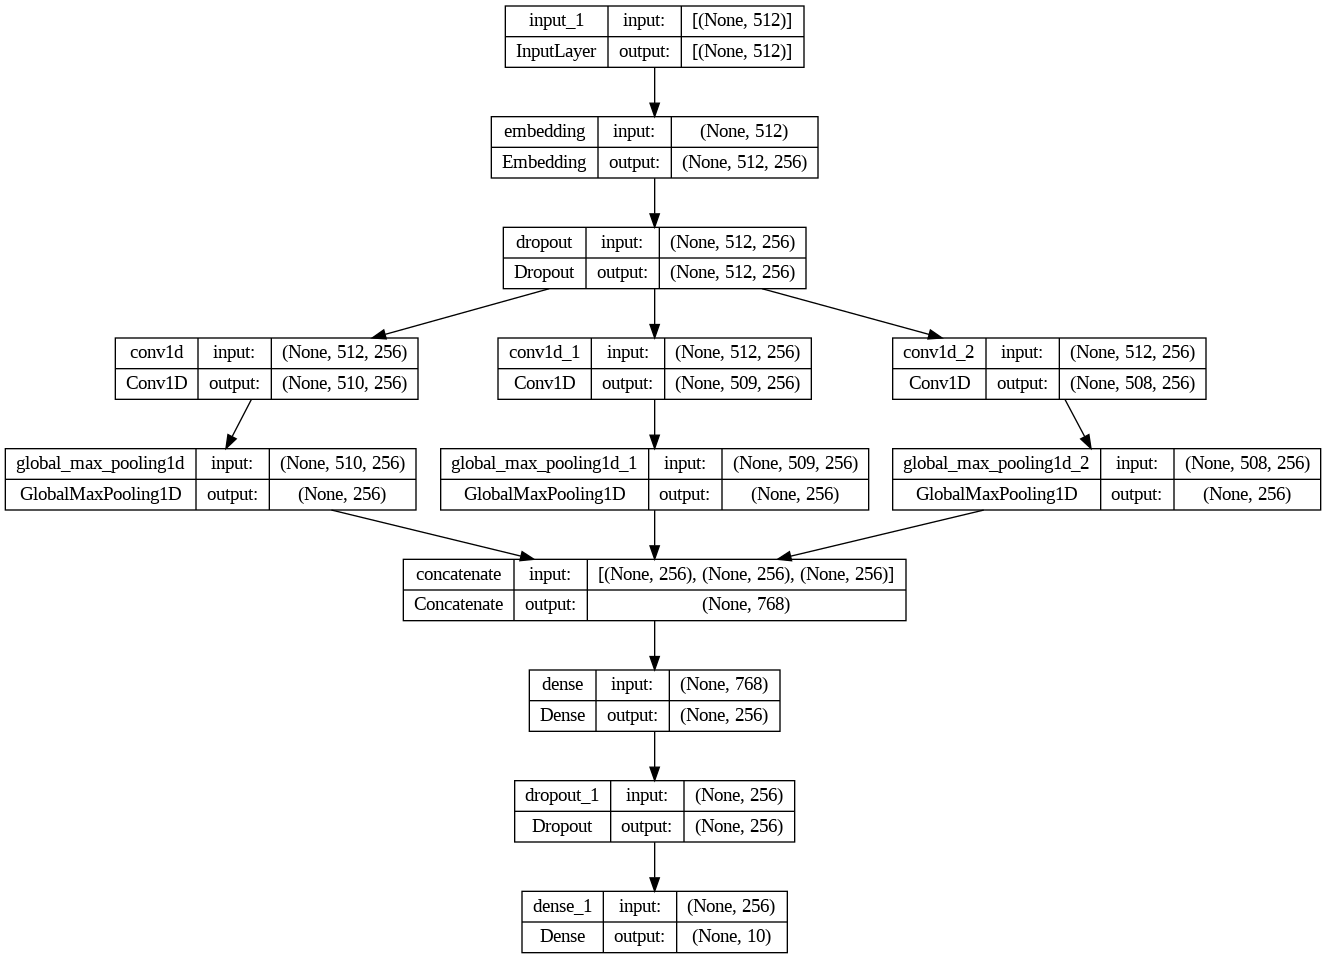
\includegraphics[width=0.85\textwidth]{MultiLayerCNN}
	\caption{Konvolūcijas neironu tīkla uzbūve - paralēla konvolūcija}
	\label{fig:MultiLayerCNN}
\end{figure}

\pagebreak
Modelis kurš apmācīts at augstākminēto arhitektūru nesiendza veiktspējas uzlabojumus, kā redzams \ref{tab:score_cnn_multi}tabulā.

\begin{table}[H]
\centering
\caption{\label{tab:score_cnn_multi}}
\textbf{Veiktspējas mēri -  konvolūcijas neironu tīkls ar parelēlu konvolūciju\\}
\begin{tabular}{|l|l|}
\hline
Akurātums & F1 \\ \hline
0.9575 & 0.9576  \\ \hline
\end{tabular}
\end{table}

\subsubsection{Priekšapstrādes nozīme}

Arī konvolūcijas neironu tīkliem tika pārbaudīta priekšapstrādes nozīme, apskatot jau minētās arhitektūras ar un bez priekšapstrādes pielietošanas Rezultāti apkopoti tabulā \ref{tab:accuracy_all_knt}, izceļot labāko rezultātu. Iespējams secināt, ka pielietojot konvolūcijas neironu tīklus, priekšapstrāde aizvien ir svarīgs solis, kas spēj pozitīvi ietekmēt modeļu klasificēšanas akurātumu.

\begin{table}[H]
\centering
\caption{\label{tab:accuracy_all_knt}}
\textbf{Akurātuma mēri dažādiem KNT modeļiem ar un bez priekšapstrādes\\}
\begin{tabular}{|l|l|l|l|}
\hline
                                      & Ar priekšapstrādi & Bez priekšapstrādes \\ \hline
KNT                                   &  \textbf{0.9617}            & 0.9533              \\ \hline
KNT + FastText                        & 0.9192            & 0.9537              \\ \hline
KNT (paralēla konvolūcija)            & 0.9575            & 0.9558               \\ \hline
KNT (paralēla konvolūcija) + FastText & 0.9058            & 0.9496 \\ \hline             
\end{tabular}
\end{table}

\pagebreak

\subsection{LSTM neironu tīkli}
LSTM tīklu implementācijai tiek veidots Keras modelis ar secīgiem slāņiem – iegulšanas, viendimensiju telpiskās atmešanas (kur atšķirībā no regulārās atmešanas aizvieto nevis nejašus elementus ar nulles vērtību, bet visas vērtības vienā dimensijā), LSTM  un pilnīgi savienotā slāņa gala klasifikācijas veikšanai. Ilustrēti ar papildus informāciju par izvēlētajām slāņu dimensijām varam apskatīt modeli \ref{fig:BaseLSTM} attēlā.

\begin{figure}[H]
\centering
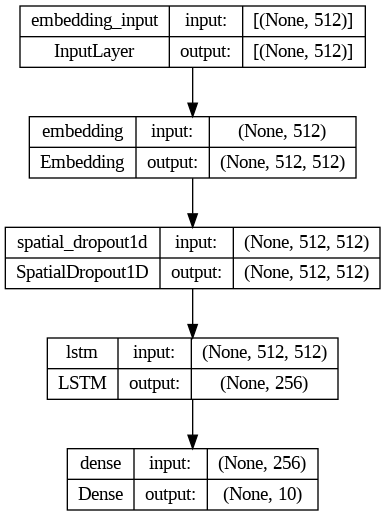
\includegraphics[width=0.4\textwidth]{BaseLSTM}
\caption{Vienkārša LSTM tīkla uzbūve}
\label{fig:BaseLSTM}
\end{figure}

Apmācība tiek veikta ar partijas izmēru kā 32, turpinot apmācību 10 epohos, saglabājot modeli posmos ar mazāko validācijas zuduma (validation loss) vērtību, mēģinot izvairīties no pārmērīgas pielāgošanas. Uz tekstiem pirms apmācības tiek veikta priekšapstrāde - simbolu un stopvārdu atmešana. Akurātuma un zuduma evolūciju pa epohiem iespējams apskatīt \ref{fig:Accuracy_Loss_LSTM_15epoch} attēlā.

\begin{table}[H]
\centering
\caption{\label{tab:score_lstm}}
\textbf{Veiktspējas mēri pielietojot LSTM neironu tīklu\\}
\begin{tabular}{|l|l|}
\hline
Akurātums & F1 \\ \hline
0.9367 & 0.9363 \\ \hline
\end{tabular}
\end{table}

Pielietojot attēlā \ref{fig:BaseLSTM} ilustrēto konvolūcijas neironu tīkla uzbūvi tiek iegūti rezultāti kā \ref{tab:score_cnn} tabulā. Pārpratuma matricu iespējams apskatīt attēlā \ref{fig:LSTM}, kur varam novērot līdzīgu kļūdu izplatību pa klasēm kā iepriekš apskatītos modeļos, arī ar šo pieeju visgrūtāk modelim ir atķirt tieši tehnoloģiju un finanšu ziņas.

\begin{figure}[H]
\centering
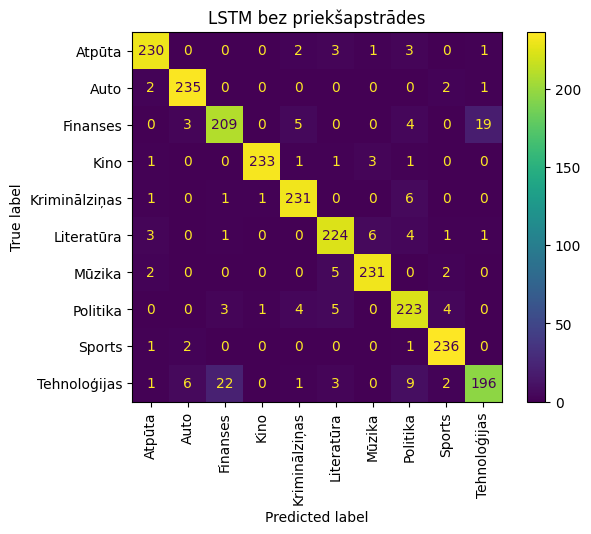
\includegraphics[width=0.75\textwidth]{LSTM}
\caption{LSTM neironu tīkls - pārpratuma matrica}
\label{fig:LSTM}
\end{figure}

\begin{figure}[H]
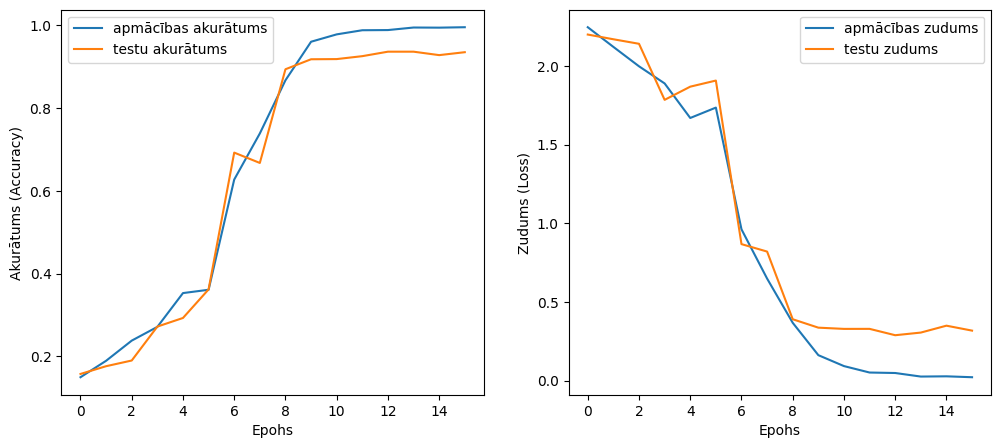
\includegraphics[width=\textwidth]{Accuracy_Loss_LSTM_15epoch}
\caption{LSTM neironu tīkls - novērtējums pa apmācības posmiem}
\label{fig:Accuracy_Loss_LSTM_15epoch}
\end{figure}

Apskatīta arī uzlabota LSTM arhitektūras pieeja, pielietojot LSTM slāņus divos virzienos, kas palīdz modelim gūt labāku konteksta un vārdu savstarpējo atkarību izpratni tekstā pirms un pēc konkrētā fragmenta.

\begin{figure}[H]
\centering
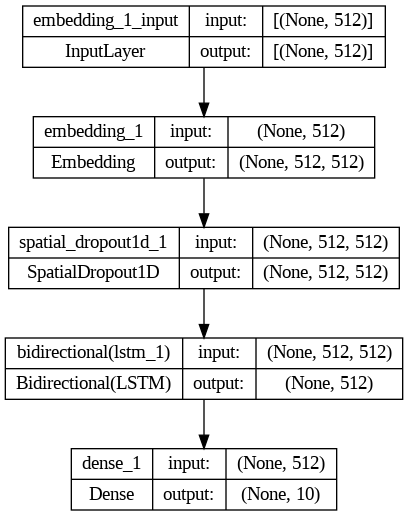
\includegraphics[width=0.4\textwidth]{BiDirectionalLSTM}
\caption{Divvirzienu LSTM neironu tīkla uzbūve}
\label{fig:BiDirectionalLSTM}
\end{figure}

Modelis kurš apmācīts at augstākminēto arhitektūru nesiendza veiktspējas uzlabojumus, kā redzams \ref{tab:score_bilstm}tabulā.

\begin{table}[H]
\centering
\caption{\label{tab:score_bilstm}}
\textbf{Veiktspējas mēri – divvirzienu LSTM\\}
\begin{tabular}{|l|l|}
\hline
Akurātums & F1 \\ \hline
0.9313 & 0.9311 \\ \hline
\end{tabular}
\end{table}

\subsubsection{Priekšapstrādes nozīme}

Arī LSTM neironu tīkliem tika pārbaudīta priekšapstrādes nozīme, apskatot jau minētās arhitektūras ar un bez priekšapstrādes pielietošanas Rezultāti apkopoti tabulā \ref{tab:accuracy_all_LSTM}, izceļot labāko rezultātu. Šo tīklu gadījumā labāki rezultāti tika sasniegti bez priekšapstrādes.

\begin{table}[H]
\centering
\caption{\label{tab:accuracy_all_LSTM}}
\textbf{Akurātuma mēri dažādiem LSTM modeļiem ar un bez priekšapstrādes\\}
\begin{tabular}{|l|l|l|l|}
\hline
& Ar priekšapstrādi & Bez priekšapstrādes \\ \hline
LSTM &  0.9329 & \textbf{0.9367} \\ \hline
Divvirzienu LSTM & 0.9304 & 0.9313 \\ \hline 
\end{tabular}
\end{table}

\pagebreak


\subsection{BERT}
Sākotnējais BERT modelis, kuru Google izstrādātāji jau bija apmācījuši un publicējuši, latviešu valodas ziņu apstrādei nav pielietojams, jo modelis apmācīts tikai uz angļu valodas tekstiem. Lai gan tikusi publicēta arī BERT uzbūves arhitektūra un modeli iespējams pašrocīgi apmācīt uz latviešu valodas tekstiem – šī darba ietvaros tas netiek veikts, jo šādai apmācībai nepieciešami ievērojami apmācības resursi ilgstošā laika posmā, kas autoram nav pieejami. Publiski gan palaik ir pieejams BERT modelis, kur apmācība uz latviešu valodas tekstiem jau ir veikta, to apmācījuši LU Matemātikas un informātikas institūta pētnieki Artūrs Znotiņš un Guntis Barzdiņš, modeli nosaucot par LVBERT. Tas ir apmācīts uz latviešu \textit{Wikipedia} ierakstiem, tekstiem no valodas korpusa LVK2018, dažādiem ziņu rakstiem un to komentāriem, kas kopā veido 500 miljonu lielu tokenu kopu apmācībai \cite{lvbert}. Salīdzinot ar sākotnējo BERT modeli, LVBERT apmācības tokenu skaits ir vairāk nekā sešas reizes mazāks.

LVBERT, gluži kā citi BERT balstītie modeļi ir vispārināti un nav piemēroti tikai vienai problēmai – tos nepieciešams pielāgot konkrētai problēmai pirms to pielietošanas, šajā gadījumā - papildus tika pievienoti slāņi tieši klasifikācijas risināšanai. Papildus tekstu priekšapstrāde netika pielietota, jo tādējādi varam pazaudēt daļu no konteksta un saiknēm starp vārdiem, kas tieši ir viena no BERT modeļu spēcīgākajām pusēm.

Modeļa pielāgošana veikta 5 epohos ar apmācības ātrumu kā 2e-5 un partijas izmēru kā 32, šai kombinācijai pēc eksperimentiem ar dažādām parametru vērtībām uzrādot labākos rezultātus. Sākotnējā BERT publikācijā \cite{devlin2019bert} pielāgošana dažādiem GLUE uzdevumiem veikta ar partijas izmēru kā 32, 3 epohos un apmācības ātrumiem 5e-5, 4e-5, 3e-5 un 2e-5 (izvēloties labāko rezultējošo modeli katram uzdevumam).  Apskatot arī citas publikācijās \cite{sun2020finetune}, kur apskatīta BERT pielāgošana teksta klasifikācijai, apmācības ātrums kā 2e-5 uzrāda labākos rezultātus, kamēr lielāki ātrumi kā 4e-4 noved pie “katastrofālas aizmiršanas” problēmas, kur iepriekš apgūtā informācija tiek zaudēta veicot jaunu apmācību.

\begin{table}[H]
\centering
\caption{\label{tab:score_bert}}
\textbf{Veiktspējas mēri pielietojot BERT\\}
\begin{tabular}{|l|l|}
\hline
Akurātums & F1 \\ \hline
0.9704 & 0.9704  \\ \hline
\end{tabular}
\end{table}

Rezultātā iegūtā modeļa raksturojošie mēri skatāmi \ref{tab:score_bert} tabulā. Lai gan salīdzinot ar citiem neironu tīklu modeļiem tiek sasniegts rezultātu uzlabojums, tas nepārsniedz atbalsta vektora mašīnu akurātumu. Angļu valodas lielie valodu modeļi pārsvarā gūst krietni labākus rezultātus klasifikācijā, salīdzinot ar vienkāršākām metodēm. Daļējs izskaidrojums LVBERT veiktspējai varētu būt ievērojami mazākais tokenu skaits apmācības posmā, salīdzinot ar angļu valodas modeli.

\begin{figure}[H]
	\centering
	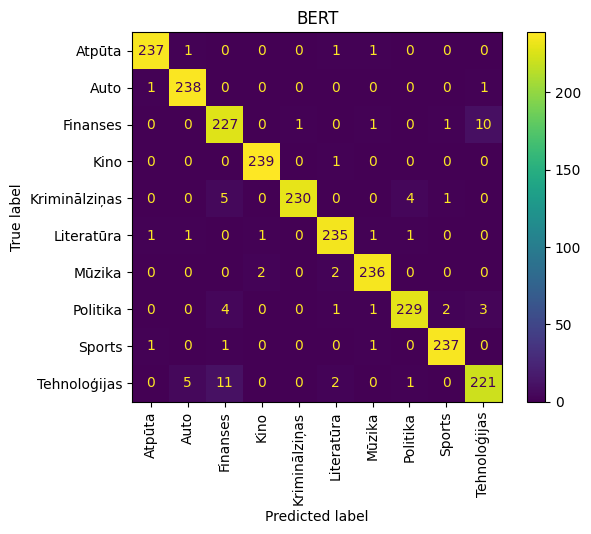
\includegraphics[width=0.75\textwidth]{Matrica_BERT}
	\caption{BERT - pārpratuma matrica}
	\label{fig:Matrica_BERT}
\end{figure}

Papildus apskatot pārpratuma matricu \ref{fig:Matrica_BERT} attēlā, BERT modelim var novērot līdzīgu klasifikācijas kļūdu sadalījums kā jau iepriekš apskatītajiem modeļiem.


%----------------------------------------------SECINĀJUMI----------------------------------------------------------

\chapter*{Secinājumi un priekšlikumi}
\addcontentsline{toc}{chapter}{Secinājumi un priekšlikumi}
Darba procesā tika noskaidrots ka ziņu klasifikācijā pielietot mašīnmācīšanās algoritmus ir noderīgi, jo iespējams veikt šo klasifikāciju ļoti precīzi, augstāko akurātuma rādītāju 0.9738 sasniedzot ar atbalsta vektora mašīnas algoritmu un TF-IDF pielietojumu pazīmju ģenerēšanā.

Novērots arī tas, ka ne visas kategorijas ir vienlīdz viegli klasificēt. Piemēram – finanšu un tehnoloģiju ziņas visiem modeļiem bija grūti klasificēt. Tas izskaidrojams ar saturisku pārklājumu starp tēmām (tehnoloģiju jaunumi un tehnoloģijas uzņēmumu finanšu jaunumi par peļņu/investīcijām).

Lai gan izpētīt un implementēt neironu tīklus un dažādas to arhitekrūtas autora ieskatā bija jēgpilni, izveidotie modeļi nespēja sasniegt augstāku precizitāti.

Autora ieskatā publiskas ziņu rakstu datu kopas ir ļoti noderīgas mašīnmācīšanās eksperimentos, piemēram, angļu valodā ziņu kopas kā “20 Newsgroup” tiek plaši pielietotas un pat iekļautas populārās bibliotēkās kā sckit-learn. Latviešu valodā šādas publiskas datu kopas netika atrastas un rakstu kopas izveide ne vienmēr ir triviāls uzdevums. Autora ievākto datu kopu publiskojot iespējama tālāka tās pielietošana citu autoru darbos.

Teksta priekšapstrāde latviešu valodā ir ierobežota morfoloģisko rīku pieejamības dēļ. Zināmus uzlabojumus priekšapstrādē autoram ir izdevies panākt ar paplašināta stopvārdu saraksta izveidi.

\textbf {Priekšlikumi:}

Autora ieskatā noderīgi būtu uzlabot modeļu apmācību ar papildus tekstu morfoloģisko apstrādi (piemēram, lemmatizāciju). Šāda apstrāde angļu un citu izplatītāku valodas tekstiem ir pieejama dažādās Python bibliotēkās, diemžēl latviešu valodas tekstiem nav tāda atbalsta. Nepieciešams veikt papildus darbu šādu rīku izstrādei.

Nepieciešama tālāka izpēte par neironu tīkliem un iespējām sasniegt augstāku precizitāti – iespējams autora izvēlētie slāņi un paramatri tīkla izveidei nebija optimāli.

Lai izvairītos no klasifikācijas problēmām kategorijās ar saturisku pārklājumu – noderīgi būtu implementēt kategorizāciju, kas spētu piešķirt tekstiem vairāk par vienas klases atbilstību. 

%---------------------------------------------LIETERATŪRA----------------------------------------------------------
\renewcommand{\bibname}{\uppercase{Izmantotās literatūras un avotu saraksts}}
\bibliographystyle{unsrt}
\bibliography{main}
\addcontentsline{toc}{chapter}{Izmantotās literatūras un avotu saraksts}

\chapter*{Galvojums}
\addcontentsline{toc}{chapter}{Galvojums}
\sloppy
\noindent Ar šo es, Matīss Kalniņš, galvoju, ka šis bakalaura darbs ir manis paša patstāvīgi 
izpildīts oriģināls darbs. Visi informācijas avoti, kā arī no tiem ņemtie dati un
definējumi ir norādīti darbā. Šis darbs tādā vai citādā veidā nav iesniegts nevienai
citai pārbaudījumu komisijai un nav nekur publicēts.

Esmu informēts (-a), ka mans bakalaura darbs tiks ievietots un apstrādāts
Vienotajā datorizētajā plaģiāta kontroles sistēmā plaģiāta kontroles nolūkos.

\vspace{1in}
\noindent202\rule{0.5cm}{0.2pt}.gada \rule{1cm}{0.2pt}.\rule{3cm}{0.2pt} \tabto{10cm} \rule{5cm}{0.2pt}
\vspace{0.5in}

Es, Matīss Kalniņš, atļauju Ventspils Augstskolai savu bakalaura darbu bez
atlīdzības ievietot un uzglabāt Latvijas Nacionālās bibliotēkas pārvaldītā datortīklā
Academia (www.academia.lndb.lv), kurā tie ir pieejami gan bibliotēkas lietotājiem,
gan globālajā tīmeklī tādā veidā, ka ikviens tiem var piekļūt individuāli izraudzītā
laikā, individuāli izraudzītā vietā.

\vspace{0.5in}
\rightline{Piekrītu \rule{4cm}{0.2pt}}
\rightline{Nepiekrītu \rule{4cm}{0.2pt}}
\vspace{0.5in}
\noindent202\rule{0.5cm}{0.2pt}.gada \rule{1cm}{0.2pt}.\rule{3cm}{0.2pt} 

\label{LastPage}
%----------------------------------------------PIELIKUMS----------------------------------------------------------

\begin{appendices}
\chapter*{Pielikums}
\renewcommand{\thesection}{\arabic{section}}
\titleformat{\section}{\normalfont\large\bfseries}{\thesection. pielikums.}{1em}{}

\section{Ar rāpuļa palīdzību izgūta raksta piemērs}
\noindent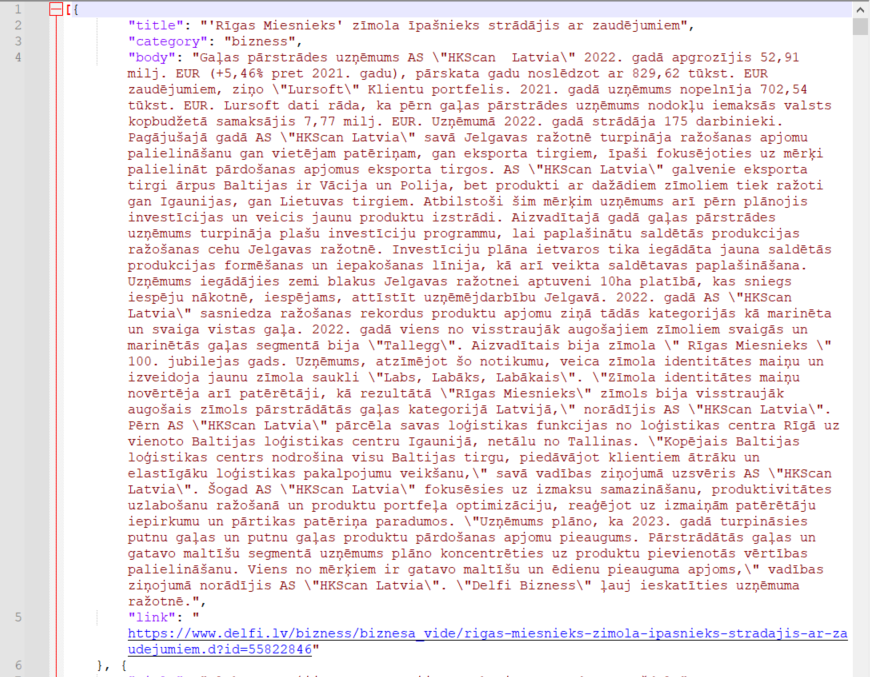
\includegraphics[width=\textwidth]{raksta_piemers}
\addtocounter{nofappendices}{1}
\label{appendix:raksta_piemers}

\section{Klasificējamo kategoriju rakstu garumi}
\noindent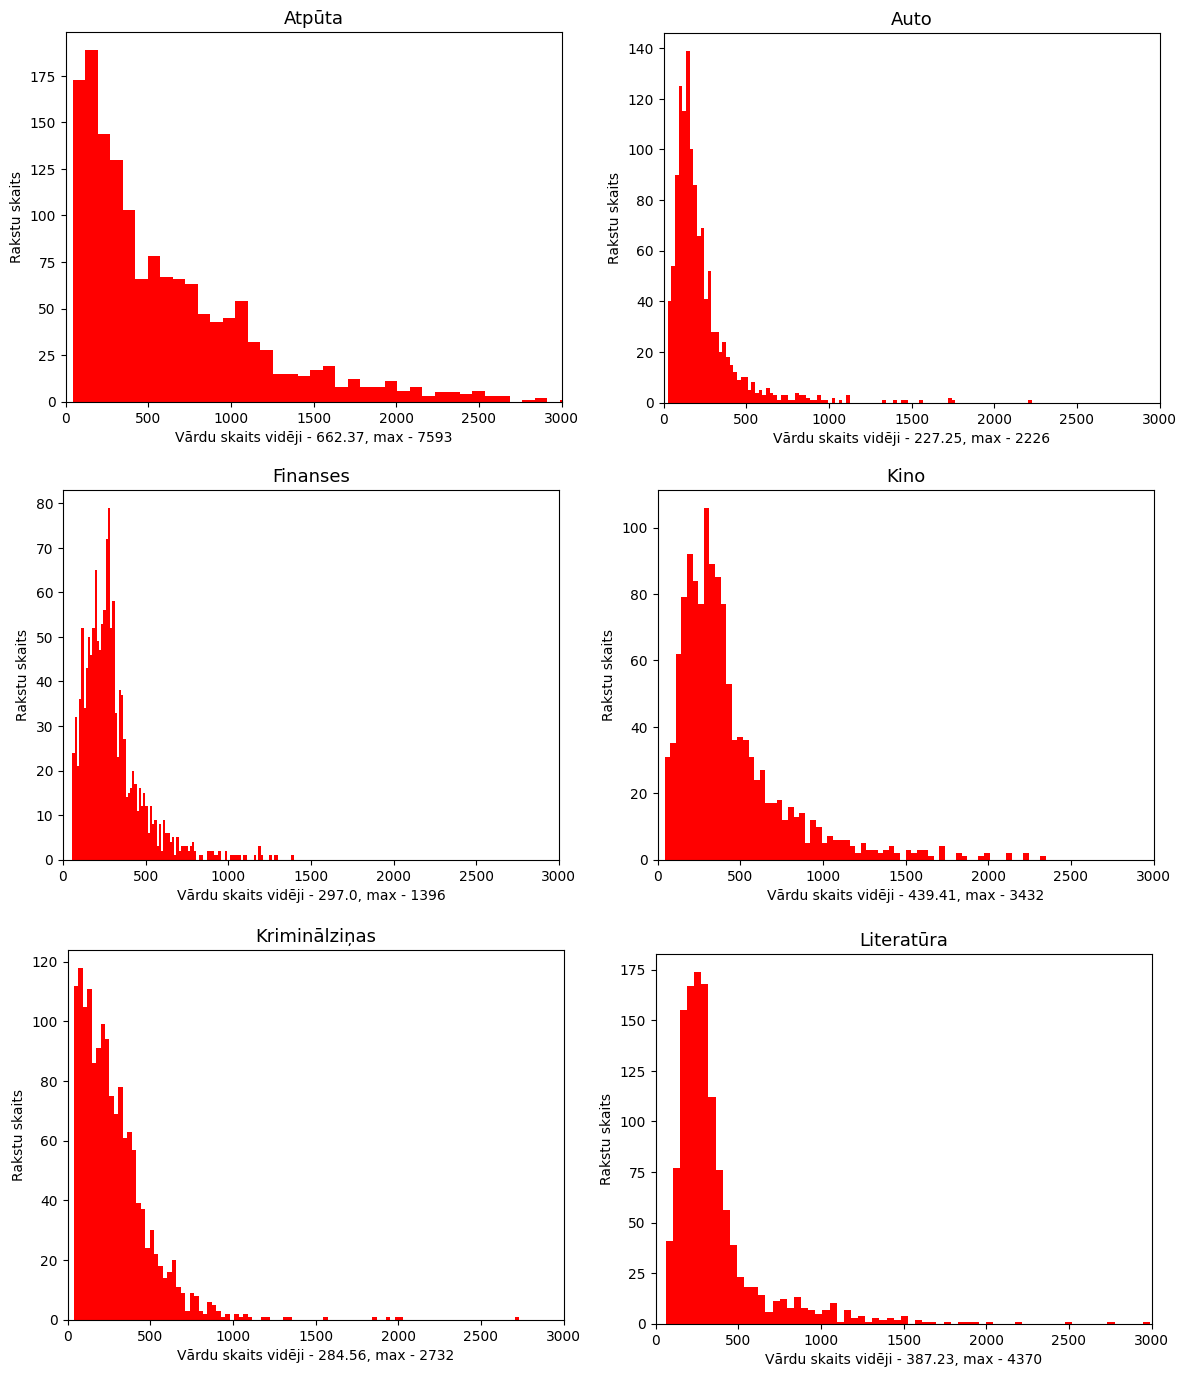
\includegraphics[width=\textwidth]{kategorijas_wc}
\noindent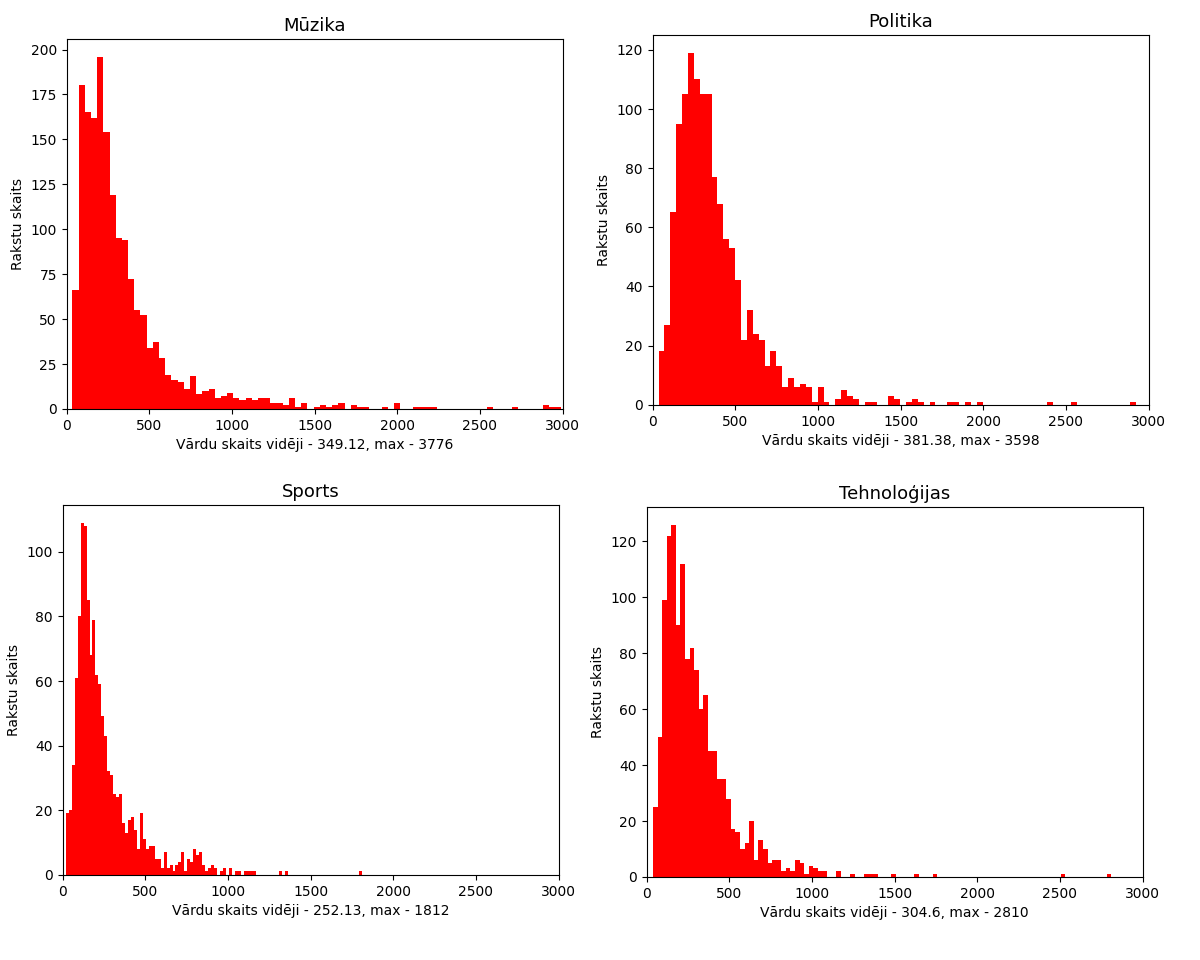
\includegraphics[width=\textwidth]{kategorijas_wc2}
\addtocounter{nofappendices}{1}
\label{appendix:kategorijas_wc}
\end{appendices}


\end{document}
